\documentclass[a4paperbi]{article}
\usepackage[utf8]{inputenc}
\usepackage[italian]{babel}
\usepackage{titling}
\usepackage{graphicx}
\usepackage{wrapfig}
\usepackage{float}
\usepackage{amsmath}
\usepackage{listings}
\usepackage[table,xcdraw]{xcolor}
\usepackage[numbers]{natbib}
\usepackage{amssymb}
\usepackage[colorinlistoftodos]{todonotes}

\renewcommand{\bibfont}{\small}
\newcommand{\HRule}{\rule{\linewidth}{0.5mm}} % Defines a new command for the horizontal lines, change thickness here

\begin{document}

\begin{titlepage}
\center % Center everything on the page
%----------------------------------------------------------------------------------------
%	HEADING SECTIONS
%----------------------------------------------------------------------------------------
\textsc{\LARGE Università degli studi di}\\[0.1cm]
\textsc{\LARGE Milano-Bicocca}\\[1.2cm] % Name of your university/college
\textsc{\Large Dipartimento di Fisica ``G. Occhialini"}\\[0.5cm] % Major heading such as course name
\textsc{\large Tesi di laurea triennale per il corso di Fisica}\\[0.5cm] % Minor heading such as course title
%----------------------------------------------------------------------------------------
%	TITLE SECTION
%----------------------------------------------------------------------------------------
\HRule \\[0.4cm]
{ \huge \bfseries Studio della Stabilità}\\[0.1cm]
{ \huge \bfseries dei Dischi di Accrescimento}\\[0.1cm]
{ \huge \bfseries  di Shakura \& Sunyaev}\\[0.4cm] % Title of your document
\HRule \\[1.5cm]
%----------------------------------------------------------------------------------------
%	AUTHOR SECTION
%----------------------------------------------------------------------------------------
\begin{minipage}{0.4\textwidth}
\begin{flushleft} \large
\emph{Autore:}\\
Riccardo Aurelio \textsc{Gilardi} % Your name
\end{flushleft}
\end{minipage}
~
\begin{minipage}{0.4\textwidth}
\begin{flushright} \large
\emph{Relatore:} \\
Prof. Massimo \textsc{Dotti} % Supervisor's Name
\end{flushright}
\end{minipage}\\[2cm]
%----------------------------------------------------------------------------------------
%	DATE SECTION
%----------------------------------------------------------------------------------------
{\large \today}\\[1cm] % Date, change the \today to a set date if you want to be precise
%----------------------------------------------------------------------------------------
%	LOGO SECTION
%----------------------------------------------------------------------------------------
	\begin{figure}[H]
		\centering
		
\includegraphics[width=0.4\linewidth]{LogoBicocca}
		\label{fig:logobicocca}
	\end{figure} % Include a department/university logo - this will require the graphicx package
%----------------------------------------------------------------------------------------
\vfill % Fill the rest of the page with whitespace
\end{titlepage}

\newpage
\clearpage\null

\newpage
\vspace*{\fill}
\textit{Ringraziamenti}\\[2cm]
\vspace*{\fill}

\newpage
\vspace*{\fill}
\tableofcontents
\vspace*{\fill}

\newpage
\section{Introduzione}
	Lo scopo di questa tesi è riassumere ed approfondire le teorie sulla stabilità delle regioni interne dei dischi di accrescimento, nel contesto del modello introdotto da Shakura e Sunyaev nel loro articolo del 1973 \textit{Black Holes in binary Systems. Observational Appearance}\footnote{\cite{ShakuraSunyaev1973}}, in riferimento alle osservazioni portate avanti per la prima volta da Lightman ed Eardley nel loro articolo del 1974 \textit{Black Holes in binary Systems: instabilityof Disk Accretion}\footnote{\cite{LightmanEardley1974}}

	Per mantenere una descrizione più semplice e meno dispersiva, ho deciso di analizzare, seguendo l'esempio di molti autori, un sistema formato da una stella ordinaria e un buco nero non rotante. Questa scelta è guidata dal fatto che il materiale in accrescimento non risente di effetti legati alla relatività generale a distanze maggiori di tre volte il raggio di Scwartzchild del buco nero
\footnote{Come dimostrato nella sezione 6.7 del \cite{FrankKingRaineAccretionPower}}. Per di più, al contrario del caso di accrescimento intorno a una stella a neutroni, il sistema in accrescimento al buco nero non sarà interessato da fenomeni legati a campi magnetici intensi. 

	Inoltre, nonostante la loro estrema compattezza permetta di apprezzare il comportamento del disco nelle sue regioni più interne, i buchi neri che fanno parte di sistemi binari sono meno semplici da osservare rispetto, per esempio, di quelli contenenti nane bianche (le cosiddette \textit{variabili cataclismiche)}.

	Va chiarito come la nostra ignoranza riguardo la natura della viscosità non ci permette di comprendere appieno il meccanismo con cui il disco irradi o come si formino i jet di materia. Sono stati costruiti molti modelli alternativi a quello standard di Shakura e Sunyaev, nei quali il disco non sia sottile in alcune regioni o non sia ovunque otticamente spesso. Ne sono esempi notevili il modello a due temperature di Shapiro, Lightman ed Eardley\footnote{descritto in \cite{ShapiroLightmanEardley1976}}, che vuole giustificare l'intensità nella regione dei raggi X dello spettro di emissione di Cygnus X-1, oppure il modello a disco coronato di Liang, che è coerente a una viscosità di origine magnetica e non puramente dinamica. Non ho potuto approfondire questi modelli nella tesi quanto avrei voluto, anche se meriterebbero molto spazio per essere analizzati. Ad oggi la teoria più promettente sulla natura della viscosità è che sia il risultato di una instabilità magneto-rotazionale (MRI)\footnote{Balbus e Hawley, 1991}.

	Prima di parlare delle instabilità nei dischi, introdurrò i concetti e le formule che descrivono un disco di accrescimento sottile, la fisica che ne governa lo stato stazionario e il meccanismo con cui si può arrivare alla sua formazione, cercando di utilizzare formule valide in generale, prima di introdurre le ipotesi di Shakura e Sunyaev.
	
\newpage
\section{Accrescimento in sistemi binari}
	L'accrescimento è uno dei processi di conversione di massa in energia tra i più efficienti nell'universo, che si sviluppa in sistemi binari di cui almeno un membro è un corpo compatto: una nana bianca, una stella a neutroni o un buco nero.

	Il travalicamento da parte di uno dei membri del sistema del suo lobo di Roche o la cattura gravitazionale da parte del corpo compatto di venti stellari emessi dal suo compagno sono particolarmente importanti tra le cause scatenanti del trasporto di materiale tra due membri di un sistema binario. Il primo di questi due processi è sicuramente meglio descritto e più semplice da trattare analiticamente e permette di dedurre delle informazioni interessanti sul meccanismo dissipativo che permette il trasporto del momento angolare. Una descrizione di questi processi permette di definire al meglio le ipotesi su cui si costruiscono i modelli di disco di accrescimento e che permettono di fare osservazioni quantitative sui sistemi.
	
	Comunque è interessante sapere che la perdita di materiale tramite venti è molto comune e particolarmente importante quando l'accrescimento avviene con tassi superiori a quelli imposti dal limite di Eddington.
	
	\begin{equation}
		\dot{M}=4\pi Gc^3\frac{m_p}{\sigma_T \eta}M
	\end{equation}
	
	Con $\sigma_T$ sezione d'urto per scattering Thomson, $m_p$ massa del protone e $\eta$ efficienza radiativa.

\subsection{Deflusso attraverso i Lobi di Roche}
	Edouard Roche ricavò la forma della struttura che ora prende il suo nome studiando l'orbita dei satelliti planetari. Descrisse il moto di alcune particelle di test immerse in un potenziale gravitazionale generato da due corpi orbitanti intorno alla loro reciproca attrazione gravitazionale.
	
	La sua costruzione è essenziale e piuttosto elegante e si può ricavare partendo da poche semplici ipotesi, prima di calcolarne numericamente i parametri. La particella di test deve avere massa abbastanza piccola, al confronto con quella dei due corpi massicci, da non poterne influenzare in modo rilevante l'orbita; le orbite sono da considerarsi kepleriane e circolari\footnote{questo non è sempre vero in pratica, ma in generale le forze mareali tendono a rendere circolari orbite eccentriche in tempi scala molto minori di quelli caratteristici di un meccanismo di trasporto di materia} e le masse sono da considerarsi condensate nel loro centro.
	
	Per descrivere qualsiasi flusso di gas tra i due corpi del sistema di massa $M_1$ e $M_2$ ha senso scrivere l'\textit{equazione di Eulero} in un sistema di riferimento co-rotante col sistema binario, con velocità angolare $\omega$ rispetto al sistema inerziale. Questo comporta la presenza nell'equazione di termini che tengano conto delle forze centrifughe e di quelle di Coriolis ($-2\omega\times\textbf{v}$), così che diventa:
	\begin{equation}
		\frac{\partial \textbf{v}}{\partial t}+(\textbf{v}\cdot\nabla)\textbf{v}=-\nabla\Phi_R-2\omega\times\textbf{v}-\frac{1}{\rho}\nabla P
	\end{equation}
	
	Con $\omega$ parallela al versore ortogonale al piano orbitale $\textbf{e}$:
	\begin{equation}
		\omega=\left[\frac{G(M_1+M_2)}{a^3}\right]^{1/2}\textbf{e}
	\end{equation}
	
	e $\Phi_R$ il \textit{Potenziale di Roche}\footnote{Immagine da \cite{FrankKingRaineAccretionPower}}, che contiene i termini relativi all'attrazione gravitazionale e le forze centrifughe (ma non quelli relativi a Coriolis):
	\begin{equation}
		\Phi_R(\textbf{r})=-\frac{GM_1}{\vert\textbf{r}-\textbf{r}_1\vert}-\frac{GM_2}{\vert\textbf{r}-\textbf{r}_2\vert}-\frac{1}{2}(\omega\times\textbf{r})^2
	\end{equation}
	
	\begin{figure}[H]
		\centering
		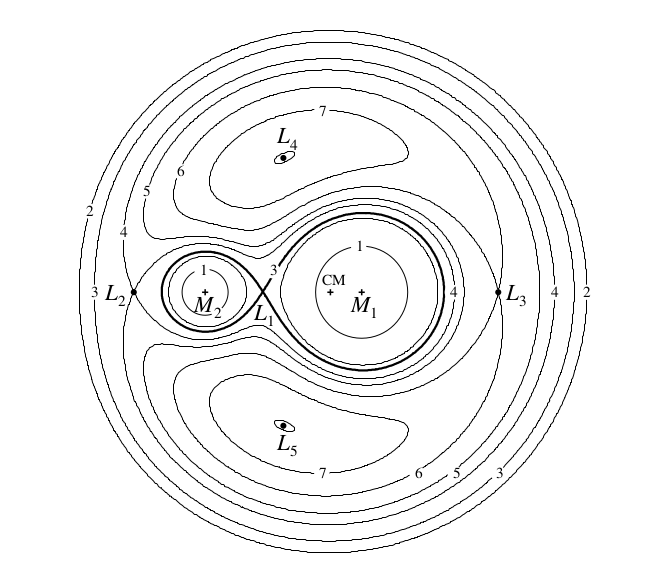
\includegraphics[width=0.6\linewidth]{RocheEquipotential}
		\caption{Una rappresentazione della sezione dei lobi e delle curve equipotenziali di $\Phi_R$. $L_1$ è il punto lagrangiano interno. Le masse sono rappresentate dai due punti neri all'interno dei lobi.}
		\label{fig:rocheequipotential}
	\end{figure}
	
	Le curve equipotenziali di $\Phi_R$ dipendono solo dal rapporto fra le masse $q=\frac{M_2}{M_1}$ e la loro scala dipende dalla distanza $a$ che le separa. Per $q\sim1$ i lobi saranno simmetrici, mentre per rapporti $q\ll1$ o $q\gg1$ avranno volumi diversi.
	
	Per distanze sufficientemente alte, la forma delle curve equipotenziali corrisponde a quella di una singola massa $M=M_1+M_2$, mentre a distanze brevi il potenziale è dominato da quello della stella più vicina. Le buche di potenziale centrate sulle posizioni dei due corpi $\textbf{r}_1$ e $\textbf{r}_2$, sono separate dalla cosiddetta \textit{superficie critica}.
	
	Il punto separatore dei due lobi, detto \textit{punto lagrangiano interno} è una sella per $\Phi_R$ tale che se del materiale in uno dei due lobi si trovasse in sua prossimità (magari a seguito dell'espansione della stella da cui proviene, che si ritroverà ad occupare tutto il volume del suo lobo), passerebbe attraverso lui per raggiungere il lobo della compagna, piuttosto che attraversare la superficie critica del potenziale.
	
	Si può trattare in maniera quantitativa la stima della geometria dei lobi e del trasporto di materia, ricavando quindi la loro dipendenza da $q$ ed $a$. E' interessante osservare che questi termini varieranno nel tempo durante qualsiasi processo di accrescimento, comportando una contrazione del lobo del corpo che sta cedendo massa ed una riduzione del periodo orbitale del sistema, insieme alla riduzione della distanza tra i due corpi, dovuta al processo di trasferimento del momento angolare nel sistema.
	
	Si può dimostrare che, nell'ipotesi di accrescimento lento e totale $\dot{M}_1+\dot{M}_2=0$, il trasferimento di materia tra i due lobi si svolge nello stesso tempo scala con cui il momento angolare viene perso.
	
	Ipotizzando sia $M_2$, che chiameremo stella secondaria, a cedere materia a $M_1$, il nostro buco nero o primaria. Con $J$ momento angolare totale del sistema, abbiamo che:
	
	\begin{equation}
		-\frac{\dot{M}_2}{M_2}=\frac{-\dot{J}/J}{4/3-M_2/M_1}
	\end{equation}
	
	e analogamente si trova che

	\begin{equation}
		\frac{\dot{a}}{a}=2\frac{\dot{P}}{3P}=\frac{2\dot{J}/3J}{4/3-q}
	\end{equation}
	
\subsection{Formazione di un disco}
	Il trasporto di materia attraverso i lobi ne aumenta anche il momento angolare, tanto da non permettere al materiale di essere accresciuto direttamente alla primaria senza che qualche meccanismo gliene faccia trasportare la maggior parte.
	
	Se il periodo orbitale del sistema non è molto lungo, il lobo primario, ovvero quello a cui viene accresciuta la materia, la vedrà provenire dal punto lagrangiano con velocità quasi completamente ortogonale alla linea dei centri, che unisce le due masse. 
	
	Definita $b_1$ la distanza tra $M_1$ e $L_1$, posso approssimare il valore della componente istantaneamente ortogonale alla linea dei centri della velocità in un sistema di riferimento inerziale con
	\begin{equation}
		v_\perp\sim b_1\omega\sim 100\,M_1^{1/3}(1+q)^{1/3}P^{-1/3}_{day}\,km\,s^{-1}
	\end{equation}  
	
	Mentre per la componente parallela, poiché immagino la forza che permette il passaggio tra i lobi della materia sia legata alla pressione, posso supporre valga
	\begin{equation}
		v_\parallel \lesssim c_{s}
	\end{equation}
	
	con $c_{s}$ velocità del suono nel lobo secondario, da cui proviene la materia. Poiché nel mezzo interstellare la temperatura ha valori $T\lesssim10^5\,K$ e poiché in generale per un gas vale $c_s\cong10(T/10^4\,K)^{1/2}km\,s^{-1}$, deve essere $v_\parallel\lesssim10\,km\,s^{-1}$
	
	Quindi in totale il moto del gas in ingresso al lobo primario deve essere supersonico. Questa condizione viene poi rinforzata dall'accelerazione che il materiale in accrescimento subirà per l'azione del campo gravitazionale del buco nero.

	\paragraph{Orbita del gas}	
	Si può dimostrare come le forze di pressione abbiano un effetto trascurabile sul materiale, che quindi si muoverà con orbita balistica nel potenziale di Roche del corpo a cui sta accrescendo, come una particella di test. Inoltre il suo moto ellittico subirà una precessione dovuta all'effetto della presenza del corpo da cui proviene.
	
	Poiché $v_\parallel\sim c_s$ è molto minore delle velocità di free-fall che le particelle acquisirebbero nell'avvicinamento a $M_1$, le condizioni iniziali all'attraversamento di $L_1$ hanno un effetto praticamente irrilevante sulla loro orbita, che sarà quindi essenzialmente unica per ogni particella di test. Queste orbite dovranno comunque intersecarsi fra loro per via della precessione a cui sono soggette tutte singolarmente. Per un flusso continuo di gas, questo comporta la dissipazione di energia termica tramite degli urti (\textit{shock}) fra le particelle che lo formano. 
	
	Attraversato $L_1$, il gas in accrescimento si troverebbe, senza un meccanismo di dissipazione, a seguire l'orbita a potenziale minore per un dato momento angolare ($R_{circ}v_\phi(R_{circ})=b_1^2\omega$), ovvero un'orbita circolare, ad un certo raggio $R_{circ}$ e con velocità circolare
	\begin{equation}
		v_\phi(R_{circ})=\left(\frac{GM_1}{R_{circ}}\right)^{1/2}
	\end{equation}
	
	E' possibile ricavare il valore del \textit{raggio di circolarizzazione} $R_{circ}$, utilizzando la formula del periodo della binaria $\omega=2\pi/P$ e si può dimostrare tramite la computazione dei parametri dei lobi come questo sia di un fattore $2\sim3$ più piccolo del raggio medio del lobo primario. Questo comporta che, a meno del caso in cui il raggio della primaria sia maggiore del raggio di circolarizzazione ($R_\star>R_{circ}$), la materia tenderebbe ad orbitare stabilmente nel lobo, una volta superata $L_1$.
	Non risulta interessante considerare l'eccezione sopracitata, poiché l'accrescimento è un processo tanto più efficiente (e quindi osservabile) tanto più sono compatti gli oggetti intorno a cui avviene: se per una nana bianca realisticamente $R_{WD}\lesssim10^9\,cm$ normalmente ci si aspetta per il raggio di circolarizzazione un valore $R_{circ}\gtrsim3.5\times10^9P_{hr}^{2/3}\,cm$.

	Un anello di materia dovrà necessariamente subire dei processi dissipativi, come degli urti, che convertiranno necessariamente parte dell'energia del moto orbitale delle particelle che lo formano in energia interna, ovvero calore. Parte di questa energia sarà irradiato con una certa efficienza $\eta$ e quindi perso dal gas, costringendo le sue particelle interessate dalla dissipazione ad avvicinarsi alla primaria (nell'ipotesi in cui risentano del solo potenziale gravitazionale del corpo massiccio). 
	
	Affinché sia conservato il momento angolare nel disco, parte del momento delle particelle che si stanno avvicinando al corpo massiccio dovrà essere trasportato verso l'esterno. Il tempo di redistribuzione del momento angolare è maggiore sia dei tempi scala di raffreddamento radiativo $t_{rad}$ che di quello orbitale (dinamico) $t_{\phi}$. Quindi parte del gas che orbitava sul raggio di circolarizzazione, perdendo energia e trasportando momento angolare, spiraleggerà lentamente verso la primaria, costretto in una serie di orbite approssimativamente circolari, nella configurazione cosiddetta di \textbf{disco di accrescimento}. 	
	
	In assenza di torsioni esterne le particelle esterne del disco a cui viene trasferito momento, dovranno quindi spiraleggiare verso l'esterno a raggi maggiori di quelli di circolarizzazione, fino a a una distanza tale per cui qualche meccanismo non gli impedisca di allontanarsi oltre\footnote{Anche se, poiché il \textit{momento angolare specifico} $h$ per materia che orbita ad un raggio $R$ vale $h=R^2\Omega\propto R^{1/2}$ e quindi tende all'infinito per raggi infiniti, nel modello la materia dovrebbe dirigersi definitivamente verso il centro del disco, con il momento che si allontana a distanze sempre maggiori trasportato da una massa sempre minore}.
		
\subsection{Processi Dissipativi}
	Per un elemento di gas di massa $m$, che stia raggiungendo l'ultima orbita stabile (Innermost Stable Circular Orbit,  $R_{\star}\equiv 3R_{sch}$) intorno al buco nero, l'energia di legame varrà $E=\frac{1}{2}\frac{GMm}{R}$. Considerando il valore di questa energia come trascurabile alla distanza da cui provengono, posso dire che la luminosità totale del disco dovrà valere
	
	\begin{equation}
		L_{disc}=\frac{GM\dot{M}}{2R_{\star}}=\frac{1}{2}L_{acc}
	\end{equation}

	Questo comporta che se metà dell'energia dall'accrescimento viene irradiata dalla materia che si muove verso l'ISCO, l'altra metà dovrà essere irradiata tutta dal bordo interno del disco. Inoltre poiché il momento angolare in funzione del raggio vale $R^2\Omega(R)\propto R^{1/2}$ e che $R_{\star}\ll R_{circ}$, il gas che forma il disco dovrà perdere quasi completamente il suo momento nella discesa verso la primaria\footnote{Immagine da \cite{ShakuraSunyaev1973}}.	
	
	Nel contesto dei dischi di accrescimento (strutture gassose con una rotazione differenziale rispetto al raggio formate da particelle con velocità circa ortogonale alla direzione radiale), ha senso supporre che il meccanismo di trasporto del momento angolare e di dissipazione dell'energia in calore sia legato alla \textit{tensione viscosa di taglio} che si esercita fra strati diversi del disco.	

	Si può capire come avvenga il trasporto di momento angolare per dissipazione viscosa considerando per esempio due strati successivi del disco di uno spessore arbitrariamente piccolo $\lambda$, separate da una superficie a che si trova a distanza $R$ dal centro del buco nero. Elementi del fluido che forma il disco, muovendosi caoticamente, potranno continuamente venire scambiati tra i due strati con velocità $\tilde{v}$. Questi elementi percorreranno in media una distanza $\lambda$ prima di interagire con elementi dello strato che hanno raggiunto e poiché la loro velocità dipendeva dal raggio a cui sono partiti, dopo una serie di scambi, ci sarà un \textit{trasporto netto di momento angolare} tra i due strati. Questo senza un trasporto netto di materia, per simmetria.

	\begin{figure}[H]
		\centering
		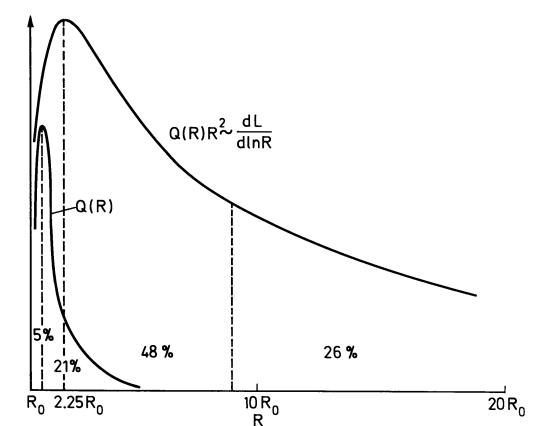
\includegraphics[width=0.8\linewidth]{LuminositaRaggio}
		\caption{Rappresentazione della luminosità emessa per raggio intorno a un disco di accrescimento. $R_0=3R_{Sch}$. $Q(R)$ è una funzione proporzionale alla luminosità e le percentuali indicano la frazione d'area del grafico nelle sezioni, separate dalla linea tratteggiata}
		\label{fig:LuminositaRaggio}
	\end{figure}

	\paragraph{Forma funzionale della viscosità}	
	Al momento non siamo ancora in grado di dare prescrizioni fisiche per la stima dei valori di $\lambda$ e $\tilde{v}$, così strettamente legati al significato fisico della dissipazione viscosa che agisce nel disco. Risultati moderni collegano la viscosità a processi magnetici, come suggerito per primi da Shakura e Sunyaev nel 1973 e sviluppato da Balbus e Hawley nel 1991, ma non esiste ancora una risposta certa o esaustiva a riguardo. 
	
	Si dimostra che in generale la densità di forza viscosa di taglio vale
	\begin{equation}
		f_{visc,taglio}\sim\rho\lambda\tilde{v}\frac{\partial^2v_\phi}{\partial R^2}\sim\rho\lambda\tilde{v}\frac{v_\phi}{R^2}
	\end{equation}

	Questo ci permette di ricavare un valore per il \textit{termine di Reynolds}, che stima l'importanza dinamica del termine viscoso rispetto a quello inerziale (ovvero $\rho(\partial\textbf{v}/\partial t+(\textbf{v}\cdot\nabla)\textbf{v})$, estratto dall'equazione di Eulero)
	\begin{equation}
		Re\sim\frac{v_\phi^2/R}{\lambda\tilde{v}v_\phi/R^2}=\frac{Rv_\phi}{\lambda\tilde{v}}
	\end{equation}
	
	Quindi possiamo dimostrare che la viscosità che permette l'accrescimento non è semplicemente quella classicamente legata ad un gas, per cui sarebbero $\lambda\sim\lambda_d$ la lunghezza minima per cui l'interazione reciproca fra le particelle del gas le deflette e $\tilde{v}\sim c_s$ velocità del suono. In questo caso, utilizzando risultati della fluidodinamica, troviamo che sarebbe $Re_{mol}\gtrsim10^4$ in regioni interne a un tipico disco di accrescimento. Questo valore implicherebbe una irrilevanza estrema del termine viscoso rispetto a quello inerziale nel disco, dimostrando che la "viscosità molecolare" non può essere responsabile del trasporto.
	
	Poiché si è dimostrata sperimentalmente l'esistenza di un \textit{numero di Reynold critico} oltre cui il moto del gas diventa turbolento, con grandi variazioni di velocità in grande e piccola scala\footnote{In particolare Lynden-Bell e Pringle hanno stimato nel loro articolo del 1974 $Re_{crit}\sim 10^3$, basandosi su esperienze in laboratorio}, si potrebbe supporre che anche nei dischi di accrescimento il processo principale di redistribuzione del momento angolare sia un moto turbolento, anche se non è stato dimostrato.
	La viscosità in questo tipo di sistema dinamico dipenderebbe da una lunghezza caratteristica dei vortici più grandi, che ci aspettiamo non poter superare l'altezza del disco $\lambda_{turb}\lesssim H$ e da una velocità degli stessi vortici che ci aspettiamo essere subsonica $v_{turb}\lesssim c_s$, tali per cui $\nu_{turb}\sim \lambda_{turb}v_{turb}$.
	Poiché non siamo ancora in grado di descrivere matematicamente un moto turbolento, né capiamo appieno i meccanismi fisici che ne regolerebbero l'intensità\footnote{Sono molti gli esempi nella letteratura sui dischi di accrescimento che spiegano come l'ipotesi del moto turbolento sia stata approfondita per capirne le possibili cause, spostando l'attenzione sulla possibilità che siano i campi magnetici a generarlo. Questo comunque attraverso il vaglio di numerose e diverse ipotesi negli anni, di cui non ho parlato per brevità.}, si è dimostrato utile, in un approccio semi-empirico all'analisi dei dischi, parametrizzare la \textit{viscosità dinamica} con
	\begin{equation}
		\nu=\alpha c_s H
	\end{equation}
	
	Questa è la cosiddetta \textit{condizione $\alpha$ di Shakura e Sunyaev}, con $\alpha\lesssim 1$ adimensionale: una parametrizzazione utile per la costruzione di un modello di disco, che riesce a sintetizzare la nostra ignoranza sulla natura della viscosità, ma non ci permette di avere un modello deterministico di disco.
	
	\paragraph{Momento torcente}
	Una frazione di fluido dallo strato più interno trasporterà in media un momento $L(R+\lambda/2)$, mentre una dallo strato più esterno trasporterà in media $L(R-\lambda/2)$. Questo trasporto netto si traduce in una \textit{torsione del disco interno su quello esterno}.
	
	Se i due strati hanno densità $\rho(R)$ e altezza $H(R)$, ci sarà un trasporto di materia netto nell'ordine di $H\rho\tilde{v}$ e per un osservatore co-rotante con il fluido che si trovi sulla superficie di separazione il \textit{momento torcente medio} che si esercitano reciprocamente per unità di angolo e al primo ordine in $\lambda$ varrebbe:
	\begin{equation*}
		-\lambda(\rho\tilde{v} H) R^2\frac{d\Omega}{dr}
	\end{equation*}
	
	E per il nostro sistema di dischi concentrici, definendo la \textit{densità superficiale} $\Sigma=H\rho$ e il \textit{coefficiente di viscosità cinematica} $\nu\sim\lambda\tilde{v}$, possiamo scrivere il \textit{momento torcente} esercitato dal disco esterno su quello interno come
	\begin{equation}
		G(R)=2\pi R\nu\Sigma R^2\frac{d\Omega}{dr}
	\end{equation}
	
	Si può apprezzare l'efficacia di questa formula nel descrivere l'accrescimento notando come si annulla nel caso di una rotazione rigida $\Omega'=\frac{d\Omega}{dr}=0$ ed è negativa nel caso in cui la velocità angolare decresca allontanandosi dal centro del disco, comportando quindi il trasporto del momento angolare dagli strati più interni verso quelli più esterni, con il conseguente spiraleggiare verso l'interno del gas.
		
	\paragraph{Energia dissipata}
	Sempre con l'analogia dell'attrito viscoso fra gli strati del disco, si può ricavare una formula per la \textit{frazione di energia dissipata} per unità di area:
	\begin{equation}
		D(R)=\frac{G\Sigma'}{4\pi R}=\frac{1}{2}\nu\Sigma(R\Omega')^2
	\end{equation}
	
	Funzione sempre positiva o nulla, nel caso della rotazione rigida, legata ovviamente all'efficacia radiativa $\eta$ del nostro sistema.
	
	La formula di $D(R)$ si ricava considerando i due momenti torcenti che agiscono ai due lati di un anello di gas che si estende tra $R$ e $R+dR$, tali per cui, se vengono divisi per la velocità angolare
	\begin{equation}
		\frac{1}{\Omega}(G(R+dR)-G(R))=\frac{1}{\Omega}\frac{\partial G}{\partial R}dR=\frac{1}{\Omega}\left[\frac{\partial}{\partial R}(G\Omega)-G\Omega'\right]dR
	\end{equation}
	
	Quest'equazione è formata da due termini, primo dei quali è $\frac{\partial}{\partial R}(G\Omega)dR$, che rappresenta il tasso di "spostamento" dell'energia nel gas per mezzo dei momenti torcenti e se integrato per tutti i raggi ha un valore che dipende solo dalle condizioni agli estremi del disco. Il secondo termine è $-G\Omega'dR$ e rappresenta un tasso di perdita locale di energia meccanica nel gas, che sarà quindi dissipata sotto forma di calore.
	
	La formula di $D(R)$ si ricava considerando che il calore sarà irradiato su entrambe le facce del disco, con superficie $4\pi RdR$.
	
\newpage
\section{Modello di Struttura del Disco Sottile}
	Definite le condizioni in cui avviene l'accrescimento e che portano alla formazione intorno al buco nero di un disco, se ne possono descrivere le proprietà e la struttura locale partendo da delle assunzioni sulla sua forma. 

	Un'ipotesi che si è rivelata particolarmente efficace nel costruire un modello semplice, come quello di Shakura e Sunyaev\footnote{Sebbene molti modelli diversi siano stati costruiti a riguardo per giustificare le osservazioni sperimentali con ipotesi diverse}, è quella che il disco sia ovunque \textit{sottile}, ovvero considerare il gas che forma il disco così strettamente confinato al piano orbitale che si può trattare come un flusso di materia quasi-bidimensionale. Questa proprietà si può anche riassumere dicendo che ci aspettiamo l'altezza del disco sia ovunque molto minore del suo raggio esterno: $H\simeq\frac{c_s}{v_\phi}R\ll R$, con $v_\phi=\left(\frac{GM}{R}\right)^{1/2}$ velocità kepleriana a distanza $R$ dal buco nero di massa $M$.
	
	Nel loro articolo seminale\footnote{\cite{ShakuraSunyaev1973}}, i due astrofisici moscoviti sono stati in grado di dimostrare come l'ipotesi di disco sottile sia precisamente equivalente a quella di raffreddamento efficiente e di orbite kepleriane, così che se una di queste manca, lo fanno tutte. Quindi si dimostra che nelle zone termicamente stabili del disco deve valere l'ipotesi di sottigliezza.
	
	Questo particolare ovviamente, per quanto semplifichi la costruzione del modello di disco, non è completamente confermato dalle osservazioni, portando alla ri-discussione del modello di disco di accrescimento per mezzo di soluzioni a due temperature e non ovunque sottil. Ha comunque senso sviluppare e descrivere il disco come sottile, per apprezzare meglio le imperfezioni nel modello che Shakura e Sunyaev hanno sviluppato a partire da questa ipotesi.
		
	\paragraph{Conservazione della massa e Densità superficiale}
		Nell'ipotesi che il materiale del disco orbiti in modo circa kepleriano, si può descrivere il suo spostamento verso il corpo in accrescimento sommando alle velocità kepleriane una componente radiale $v_R$, negativa in un sistema di riferimento centrato su $M$ in coordinate polari.

	Considerando ancora un anello di gas da $R$ a $R+dR$, la cui massa vale $2\pi RdR\Sigma$ e che ha momento angolare totale $2\pi RdR\Sigma R^2\Omega$. Il flusso netto tra anelli vicini è descritto dalla variazione di queste due quantità. 
	
	Per la massa
	\begin{align*}
		\frac{\partial}{\partial R}(2\pi RdR\Sigma)&=v_R(R,t)2\pi R\Sigma(R,t)-v_R(R+dR,t)2\pi(R+dR)\Sigma(R+dR,t)\\
		&\cong-2\pi dR\frac{\partial}{\partial R}(R\Sigma v_R)
	\end{align*}
	
	Che nel limite $dR\rightarrow 0$ è l'\textit{equazione di conservazione della massa} nel disco
	\begin{equation}
		R\frac{\partial\Sigma}{\partial t}+\frac{\partial}{\partial R}(R\Sigma v_R)=0
	\end{equation}
	
	Analogamente partendo da
	\begin{equation*}
		\frac{\partial}{\partial R}(2\pi RdR\Sigma R^2\Sigma)\cong-2\pi dR\frac{\partial}{\partial R}(R\Sigma v_R R^2\Sigma)+\frac{\partial G}{\partial R}dR	
	\end{equation*}
	
	Trovo che nel limite $dR\rightarrow 0$ diventa \textit{l'equazione di conservazione del momento angolare nel disco}
	\begin{equation}
		R\frac{\partial}{\partial t}(\Sigma R^2\Omega)+\frac{\partial}{\partial R}(R\Sigma v_R\cdot R^2\Omega)=\frac{1}{2\pi}\frac{\partial G}{\partial R}
	\end{equation}
	
	Usando la definizione di $G(R)$ e della velocità angolare in un'orbita kepleriana $\Omega_K$,  questa ci permette di definire un'equazione differenziale di $\Sigma$ ed $R$
	\begin{equation}
		\frac{\partial\Sigma}{\partial t}=3R^{-1}\frac{\partial}{\partial R}\left\{R^{1/2}\frac{\partial}{\partial R}\left[\nu\Sigma R^{1/2}\right]\right\}
	\end{equation}
	
	In generale, supponendo $\nu$ sia una funzione delle condizioni locali del disco (ovvero di $\Sigma$, $R$ e $t$), questa rappresenta un'equazione non lineare di diffusione di $\Sigma$, ma supponendo che $\nu$ sia funzione del solo raggio e scali come una sua potenza, l'equazione diventa lineare e risolvibile analiticamente. In particolare nel caso in cui $\nu$ sia costante, come assunto nel modello di Shakura-Sunyaev, la soluzione per un disco che va da $R=0$ a $R=\infty$ e momento torcente nullo all'origine è ricavabile analiticamente e vale\footnote{Questa dimostrazione si deve a Lüst (1954)}\footnote{Nel caso in cui sia $\nu\propto\Sigma^aR^b$, il sistema è comunque risolvibile analiticamente. Il caso con $a=3/7$ e $b=15/14$ corrisponde al caso di un disco otticamente spesso di SeS}
	\begin{equation*}
		\Sigma(R,t)=(12)^{1/4}R^{-3/4}\nu^{-3/4}\int^{\infty}_0d\lambda\,f(\lambda)e^{-\lambda^2t}J_{1/4}(R\lambda/\sqrt{3\nu})(R\lambda/\sqrt{3\nu})^{1/4}
	\end{equation*}
	
	Dove $f(\lambda)$ è una funzione che dipende dalle condizioni iniziali e $J_{1/4}$ è la funzione ordinaria di Bessel di ordine $1/4$.
	
	La soluzione corrispondente alla distribuzione iniziale di materia sul disco è l'\textit{equazione di Green} per un anello di massa $m$ che si trovava inizialmente ad un raggio $R_0$, che mi aspetto essere intorno a $R_{circ}$
	\begin{equation}
		\Sigma(R,t=0)=\frac{m}{2\pi R_0}\delta(R-R_0)
	\end{equation}
	
	Posso scrivere questa soluzione implicitamente, definendo i due parametri adimensionali $\chi=R/R_0$ e $\tau=12\nu tR_0^{-2}$, come funzione di $\chi$ per diversi $\tau$:
	\begin{equation}
	\Sigma(\chi,\tau)=\frac{m}{\pi R_0^2}\tau^{-1}\chi^{-1/4}exp\left\{-\frac{1+x^2}{\tau}\right\}I_{1/4}(2\chi/\tau)
	\end{equation}
	
	$I_{1/4}$ è la funzione di Bessel modificata.
	
	Ponendo $(1+\chi^2)\tau^{-1}\sim 1$, questa equazione ci mostra come la viscosità influenzi la densità superficiale originale in un \textit{tempo scala viscoso} o \textit{di scivolamento radiale} $t_{visc}\sim R^2/\nu$ e anche che $\tau\sim t/t_{visc}(R_0)$.
	
	Il tempo scala si può chiamare di "scivolamento radiale", perché l'equazione usata per derivare $\frac{\partial\Sigma}{\partial t}$ permette anche di derivare una funzione per le velocità radiali
	\begin{equation}
		v_R=-\frac{3}{\Sigma R^{1/2}}\frac{\partial}{\partial R}(\nu\Sigma R^{1/2})
	\end{equation}
	
	Tale per cui $v_R\sim\frac{\nu}{R}\sim\frac{R}{t_{visc}}$.
	
	Costruendo un grafico della densità di superficie nel tempo\footnote{Immagine da \cite{Pringle1981}} si può notare come questa si evolva dall'anello ad $R_0\sim R_{circ}$ in una distribuzione asimmetrica, più alta verso il centro del disco che verso il suo esterno, dove comunque parte della materia si dirige per la conservazione del momento angolare totale.
	
	\begin{figure}[H]
		\centering
		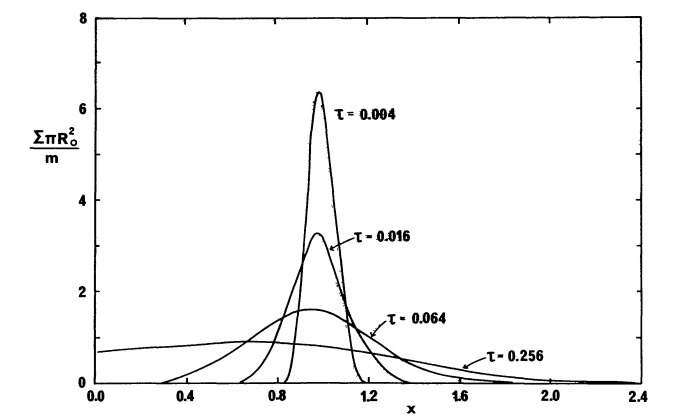
\includegraphics[width=0.7\linewidth]{DensSuper}
		\caption{Evoluzione viscosa di un disco di materia di massa $m$ in funzione di $x=R/R_0$, con $\tau=12\nu t/R_{circ}^2$.}
		\label{fig:denssuper}
	\end{figure}

	Questo risultato è reso evidente analiticamente se si considera che, poiché il comportamento asintotico dell'equazione modificata di Bessel è
	\begin{equation*}
		I_{1/4}(z)\propto\begin{cases}
				z^{-1/2}e^z\text{ per $z\gg1$}\\
				z^{1/4}\text{ per $z\gg1$}
			\end{cases}
	\end{equation*}
	 
	allora per la velocità radiale dovrà valere
	\begin{equation*}
		v_R\sim\begin{cases}
			\frac{3\nu}{R_0}\left\{\frac{1}{4\chi}+\frac{2\chi}{\tau}-\frac{2}{\tau}\right\}\text{ per $2\chi\gg\tau$}\\
			-\frac{3\nu}{R_0}\left\{\frac{1}{2\chi}-\frac{2\chi}{\tau}\right\}\text{ per $2\chi\ll\tau$}			
			\end{cases}
	\end{equation*}
	
	E quindi le regioni più esterne ($2\chi\gg\tau$) si muoveranno verso l'esterno, trasportando momento angolare che hanno ricevuto dalle regioni più interne, che si muovono verso il corpo in accrescimento.
	
	Il punto esatto del disco in cui la velocità radiale cambia segno si sposta, al variare del rapporto $\chi/\tau$, che possiamo considerare decrescente nel tempo. Questo perché il momento angolare sarà trasportato verso l'esterno da una frazione di massa sempre minore, col procedere dell'accrescimento.
	
\subsection{Modello di disco stazionario}
	Poiché intorno ai sistemi in accrescimento le condizioni esterne variano con tempi molto maggiori di $t_{visc}$, per tempi relativamente lunghi si può considerare la struttura del disco come stazionaria.
	
	Analizzare un modello stazionario del disco permette di derivarne diverse proprietà interessanti. Nel loro primo articolo Shakura e Sunyaev si sono occupati principalmente dell'analisi di struttura sotto questa ipotesi, senza approfondire completamente il problema dell'instabilità e dell'evoluzione temporale del modello, ripreso da Lightman ed Eardley nel loro articolo del 1974\footnote{\cite{LightmanEardley1974}}.
	
	\paragraph{Condizioni sul tasso di accrescimento}
	Considerando l'ipotesi di stazionarietà, la conservazione della massa diventa un'equazione differenziale in $R$, con soluzione
	\begin{equation}
		R\Sigma v_R=costante
	\end{equation}
	
	con la costante che rappresenta il flusso costante di materia in accrescimento
	\begin{equation}
		\dot{M}=2\pi R\Sigma(-v_R)
	\end{equation}
	
	E' importante notare come la costanza del flusso di materia sia una conseguenza diretta dall'assunzione sulla viscosità. Modelli moderni di accrescimento intorno a corpi compatti stanno considerando anche l'ipotesi che in certe sezioni del disco, $\dot{M}$ sia una funzione del raggio.
	
	La conservazione del momento angolare permette invece di derivare, una condizione sul tasso di accrescimento $\dot{M}$ rispetto alla distanza dal centro del disco.
	
	Imponendo la stazionarietà si trova:
	\begin{equation}
		\Sigma v_RR^3\Omega=\frac{1}{2\pi}(G+cost)
	\end{equation}
	
	Che per la definizione di $G(R)$ diventa
	\begin{equation}
		-\nu\Sigma\Omega'=\Sigma(-v_R)\Omega+\frac{cost}{2\pi R^3}
	\end{equation}
	
	C'è una relazione tra la costante ed il tasso di trasporto del momento angolare nel disco ed è esplicitabile con alcune considerazioni: in una situazione reale, nonostante possiamo ipotizzare che le velocità del materiale nel disco seguano orbite kepleriane e quindi che siano più veloci avvicinandosi al buco nero, deve esserci una regione "cuscinetto" di spessore $b$ in cui il materiale del disco sia rallentato per venire accresciuto al corpo centrale. Quindi deve esistere un raggio $R=R_{\star}+b$ dove $\Omega'=0$.

	Trovo che il valore della costante a $R=R_{\star}+b$, esplicitando nell'equazione della conservazione del momento le definizioni di $G(R)$ ed $\dot{M}$, diventa
	\begin{equation*}
		C=2\pi R_{\star}^3\Sigma v_R\Omega(R_{\star}+b)\vert_{R_{\star}+b}
	\end{equation*}
	
	e ponendo $\Omega(R_{\star}+b)=\left(\frac{GM}{R_{\star}^3}\right)^{1/2}[1+O(b/R_{\star})]$ diventa, per termini di ordine $b/R_{\star}$:
	\begin{equation}
		C=-\dot{M}(GMR_{\star})^{1/2}
	\end{equation}	

	Questa, sostituita nell'equazione della conservazione del momento angolare, con $\Omega=\Omega_K$, porta alla condizione su $\dot{M}$
	\begin{equation}
		\nu\Sigma=\frac{\dot{M}}{3\pi}\left[1-\left(\frac{R_{\star}}{R}\right)^{1/2}\right]
	\end{equation}
	
	Nel caso in cui valga $b\approx R_{\star}$, l'approssimazione di disco sottile non sarà più valida da $R=R_{\star}+b$ ad $R_{\star}$ e piuttosto che un anello in cui il materiale rallenta, il disco collasserà ad una conformazione "spessa".
	
	Quello che si osserva il più delle volte è invece che $b\ll R_{\star}$\footnote{Le condizioni per cui questo valga sono descritte nella sezione 6.2 del \cite{FrankKingRaineAccretionPower}}.	
	
	\begin{figure}[H]
		\centering
		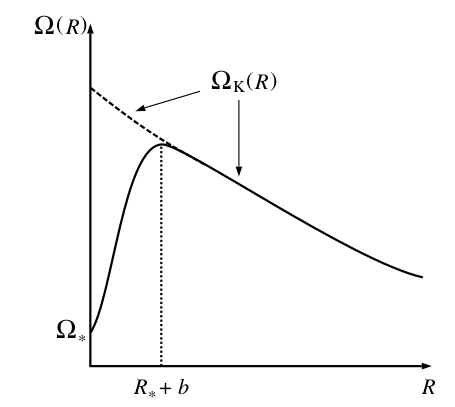
\includegraphics[width=0.7\linewidth]{InnerRegionAngularVelocity}
		\caption{Distribuzione delle velocità angolari $\Omega(R)$ intorno a una stella con $R_{\star}=R_\star$ e velocità di rotazione $\Omega_{\star}<\Omega_K(R)$}
		\label{fig:InnerRegionAngularVelocity}
	\end{figure}
	
	\paragraph{Dissipazione di energia}
	La stazionarietà del disco, nel caso di un corpo centrale che ruota lentamente permette anche di descrivere esplicitamente la dissipazione per unità d'area senza farla dipendere dalla viscosità. Ponendo $\Omega=\Omega_K$, si trova infatti:
	\begin{align}
		D(R)&=\frac{1}{2}\nu\Sigma(R\Omega')^2
			\\&=\frac{3GM\dot{M}}{8\pi R^3}\left[1-\left(\frac{R_{\star}}{R}\right)^{1/2}\right]
	\end{align}	
	
	Con questa funzione siamo in grado di calcolare la luminosità emessa da un anello del disco
	\begin{equation}
		L(R_1,R_2)=2\int_{R_1}^{R_2}D(R)2\pi RdR
	\end{equation}
	
	Che per $R_1=R_{\star}$ e $R_2\to\infty$ equivale alla luminosità di tutto il disco
	\begin{equation}
		L_{disco}=\frac{GM\dot{M}}{2R_{\star}}=\frac{1}{2}L_{acc}
	\end{equation}
	
	\paragraph{Struttura verticale del disco}
	In coordinate cilindriche, poiché non c'è ragione per credere nel disco sia presente un meccanismo che permetta del trasporto verticale di materia, lungo questa direzione deve essere mantenuto l'equilibrio idrostatico, ricavabile come parte della componente $z$ dell'equazione di Eulero:
	\begin{equation*}
		\frac{1}{\rho}\frac{\partial P}{\partial z}=\frac{\partial}{\partial z}\left[\frac{GM}{(R^2+z^2)^{1/2}}\right]
	\end{equation*}
	
	Nell'ipotesi di disco sottile ($z\ll R$) questa diventa
	\begin{equation}
		\frac{1}{\rho}\frac{\partial P}{\partial z}=-\frac{GMz}{R^3}
	\end{equation}
	
	Se definiamo una scala tipica per le altezze del disco $H$ tale per cui ovunque sul disco $z\sim H$, possiamo dire che approssimativamente $\partial P/\partial z\sim P/H$. Inoltre potrò scrivere $P\sim c_s^2\rho$.

	Questi fattori insieme comportano che
	\begin{equation}
		H\cong c_s\left(\frac{R^3}{GM}\right)^{1/2}
	\end{equation}

	Quindi la condizione di disco sottile $H\ll R$ sarà rispettata se la velocità angolare, che si può dimostrare essere molto vicina a quella kepleriana per il disco sottile, è ampiamente supersonica
	\begin{equation}
		v_\phi(R)=\left(\frac{R}{GM}\right)^{1/2}\gg c_S
	\end{equation}

	Questa è definitivamente una condizione sulla temperatura del disco e per poterla verificare in ogni punto serve un'analisi locale.
	
	Si può dimostrare analogamente che la velocità radiale è ampiamente subsonica per il disco, usando poche definizioni
	\begin{equation}
		v_R\sim\frac{\nu}{R}\sim\alpha c_s\frac{H}{R}\ll c_s
	\end{equation}
	
	\paragraph{Temperatura e Pressione} Poiché sotto l'ipotesi di disco sottile i gradienti in pressione e temperatura sono praticamente solo verticali, si può tralasciare l'analisi della componente radiale di queste grandezze (tranne che per la definizione di $D(R)$) semplificando così la descrizione del disco.
	
	Posso verificare che la condizione di equilibrio idrostatico, per un profilo verticale di temperatura costante, implica che valga
	\begin{equation*}
		\rho(R,z)=\rho_c(R)e^{-z^2/2H^2}
	\end{equation*}
	con $\rho_c$ densità del piano centrale del disco $z=0$.
	
	Quindi assumendo la temperatura centrale del disco sia $T_c(R)=T(R,0)$, posso approssimare la densità centrale di un disco con $\rho=\Sigma/H$, dove $H=Rc_s/v_\phi$ e la velocità del suono è data da $c_s^2=P/\rho$, con $P$ la somma della pressione radiativa e di quella gassosa
	\begin{equation}
		P=\frac{\rho\kappa T_c}{\mu m_p}+\frac{4\sigma}{3c}T_c^4
	\end{equation}
	
	L'equazione della temperatura centrale deve dipendere analogamente da una relazione che leghi il flusso di energia verticale e il tasso di energia generata dai processi di dissipazione viscosi. Per poter costruire un modello dettagliato del disco è utile studiarne la struttura come se fosse formata da delle atmosfere stellari ad ogni raggio. 
	
	Analogamente al caso stellare potremmo quindi chiederci se il tipo di trasporto sia  radiativo o convettivo. Studiando l'adiabaticità del sistema, si osserva che in molti casi il meccanismo di trasporto è quello radiativo. In questo caso il flusso energetico attraverso le superfici del disco vale, a z costante
	\begin{equation}
		F(z)=-\frac{16\sigma T^3}{3\kappa_R\rho}\frac{\partial T}{\partial z}
	\end{equation}
	
	Con $\kappa_R$ opacità media di Rosseland
	\footnote{Opacità media per un sistema con diversi termini sorgenti di opacità (bb,bf,ff,...)\begin{equation}
																							\frac{1}{k_R}=\frac{\int_0^\infty\frac{1}{k_\nu}\frac{\partial B_\nu(T)}{\partial T}d\nu}{\int_0^\infty\frac{\partial B_\nu(T)}{\partial T}d\nu}
																						\end{equation}}.
Questa definizione del flusso corrisponde implicitamente alla condizione che il disco sia \textit{otticamente spesso}\footnote{Sono stati costruiti anche modelli che consideravano il caso in cui il disco fosse stato otticamente sottile o la dissipazione di momento fosse accaduta in parti otticamente sottili del disco, ma la loro geometria è diversa dal caso del disco otticamente spesso. I modelli moderni di disco di accrescimento sono spesso formati da entrambi i tipi di regioni, otticamente spesse o sottili, per giustificare i flussi osservati.}, ovvero che valga
	\begin{equation}
		\tau=\rho H\kappa_R(\rho,T_c)=\Sigma\kappa_R\gg 1
	\end{equation}
	
	Questo affinché l'approssimazione a corpo nero sia valida e quindi la radiazione non sia libera di scappare dalle regioni interne in cui viene generata.
	
	Dalla definizione di flusso posso costruire un'equazione del bilancio energetico
	\begin{equation}
		\frac{\partial F}{\partial z}=Q^+
	\end{equation}

	Con $Q^+$ energia prodotta tramite processi viscosi, per unità di volume.
	
	Integrando quest'equazione trovo che
	\begin{equation}
		F(H)-F(0)=\int_0^HQ^+(z)dz=D(R)
	\end{equation}

	E poiché $F(z)\sim(4\sigma/3\tau)T^4(z)$, nell'ipotesi che la temperatura superficiale del disco sia molto minore di quella centrale $T_c^4\gg T^4(H)$
	possiamo derivare il risultato
	\begin{equation}
		\frac{4\sigma}{3\tau}T^4_c=D(R)
	\end{equation}
	
	Quindi la struttura del disco sottile che è stato possibile derivare solo usando leggi fondamentali è descritta dalle seguenti espressioni:
	\begin{equation}
	\begin{cases}
		1.\quad \rho=\Sigma/H\\
		2.\quad H=c_sR^{3/2}/(GM)^{1/2}\\
		3.\quad c_s^2=P/\rho\\
		4.\quad P=\frac{\rho\kappa T_c}{\mu m_p}+\frac{4\sigma}{3c}T_c^4\\
		5.\quad \frac{4\sigma}{3\tau}T^4_c=\frac{3GM\dot{M}}{8\pi R^3}\left[1-\left(\frac{R_{\star}}{R}\right)^{1/2}\right]\\
		6.\quad \tau=\rho H\kappa_R(\rho,T_c)=\tau(\Sigma,\rho,T_c)\\
		7.\quad \nu\Sigma=\frac{\dot{M}}{3\pi}\left[1-\left(\frac{R_{\star}}{R}\right)^{1/2}\right]\\
		8.\quad \nu=\nu(\rho,T_c,\Sigma,\alpha,...)		
	\end{cases}
	\end{equation}
		
\subsection{La soluzione di Shakura e Sunyaev}
	Per poter risolvere il sistema delle equazioni della struttura del disco stazionario di accrescimento sono necessarie una prescrizione sulla viscosità dinamica e una definizione dell'opacità del disco. Nikolai Shakura e Rashid Sunyaev sono riusciti, a trovare una soluzione semplice ed elegante al problema, con la loro \textit{condizione} $\alpha$:
	\begin{equation}
		\nu=\alpha c_sH
	\end{equation}
Questa è una legge che semplifica la forma dell'equazione della densità superficiale del disco, che ha avuto diversi riscontri sperimentali (soprattutto nei primissimi anni dello studio dei sistemi binari), ma più di tutto che è riuscita a marginalizzare la gravità della nostra ignoranza riguardo la natura dei processi viscosi nel disco, parametrizzandoli e riducendo le incognite da studiare ad una sola (la costante $\alpha$). L'altra faccia della medaglia di questa semplificazione nell'analisi delle equazioni e il vero grande problema della teoria dei dischi di accrescimento, come già detto, è che il modello di Shakura e Sunyaev (SeS), non appoggiandosi ad osservazioni fisiche, è sterile e non permette di fare previsioni. Siamo solo in grado di confrontare i risultati delle nostre osservazioni con il valore che ci aspettiamo assuma $\alpha$, per provare a capirne la natura.

Ad oggi il modello di Shakura e Sunyaev non può dirsi sicuramente affidabile, per lo meno per descrivere alcune regioni del disco. Gli sforzi dei modellisti si sono spostati da questa semplificazione verso la ricerca di una soluzione fisicamente stabile e coerente con le osservazioni dei sistemi binari che conosciamo.

Per quanto riguarda l'opacità, SeS hanno assunto che la densità $\rho$ e la temperatura centrale $T_c$ fossero tali che l'opacità media di Rosseland fosse approssimabile con la legge di Kramer
\begin{equation}
	k_R=6.6\times10^{22}\rho T_c^{-7/2}\,cm^2g^{-1}
\end{equation}
e hanno inoltre deciso di trascurare il termine legato alla pressione di radiazione nella formula di $P$.

Con queste ipotesi si ottiene la soluzione del sistema, scritta in termini di $R_{10}=R/(10^{10}\,cm)$, $M_{1}=M/(M_\odot)$, $\dot{M}_{16}=\dot{M}/(10^{16}\,g\,s^{-1})$ e con $f=\left[1-\left(\frac{R_*}{R}\right)^{1/2}\right]^{1/4}$. 

Poniamo inoltre $\mu=0.615$, valore atteso per un medium completamente ionizzato formato da diversi gas. 

\begin{equation}
	\begin{cases}
		\Sigma=5.2\,\alpha^{-4/5}\dot{M}_{16}^{3/20}M^{1/4}_1R_{10}^{-3/4}f^{14/5}\,g\,cm^{-2}\\
		H=1.7\times10^8\alpha^{-1/10}\dot{M}^{3/20}_{16}M^{-3/8}_1R_{10}^{9/8}f^{3/5}\,cm\\
		\rho=3.1\times10^{-8}\alpha^{-7/10}\dot{M}^{11/20}_{16}M^{5/8}_1R_{10}^{-15/8}f^{11/5}\,g\,cm^{-3}\\
		T_c=1.4\times10^{4}\alpha^{-1/5}\dot{M}^{3/10}_{16}M^{1/4}_1R_{10}^{-3/4}f^{6/5}\,K\\
		\tau=33\,\alpha^{-4/5}\dot{M}^{1/5}_{16}f^{4/5}\\
		\nu=1.8\times10^{14}\alpha^{4/5}\dot{M}^{3/10}_{16}M^{-1/4}_1R_{10}^{3/4}f^{6/5}\,g\,s^{-1}\\
		v_R=2.7\times10^{14}\alpha^{4/5}\dot{M}^{3/10}_{16}M^{-1/4}_1R_{10}^{-1/4}f^{-14/5}\,cm\,s^{-1}\\
	\end{cases}
\end{equation}

	Questo sistema di soluzioni rappresenta, per parametri ragionevoli, un disco sottile con $H/R=1.7\times10^8\alpha^{-1/10}\dot{M}^{3/20}_{16}M^{-3/8}_1R_{10}^{1/8}f^{3/5}$, la cui velocità radiale è subsonica $v_R\sim 0.3\,km\,s^{-1}$ ($c_s\sim10\,km\,s^{-1}$) e la cui velocità kepleriana è ampiamente supersonica $v_\phi\sim1000\,km\,s^{-1}$. Inoltre il disco risulta essere otticamente spesso e praticamente uniforme nella direzione verticale poiché sia $T_c$ che $T(R)$ sono nell'ordine di $\sim\tau^{1/4}\sim2$.

	Anche ipotizzando il nostro valore di $\alpha$ sia mediato verticalmente e, data l'uniformità del sistema, ignorandone quindi la dipendenza da $z$, resta purtroppo nulla la nostra conoscenza sulle sue dipendenze da $R$, $M$, $\dot{M}$ e dal tempo.
	E' evidente come $\alpha$ non compaia nella soluzione con grandi potenze e quindi il suo ordine di grandezza risulti poco rilevante sui risultati delle equazioni di struttura, ma questo significa contemporaneamente che difficilmente potremo stimarne il valore con precisione solo attraverso osservazioni dirette di sistemi binari. 	
	Se si può dire che si ottengono valori realistici dei parametri d'accrescimento dal modello per $\alpha\lesssim1$, sicuramente non ci sono elementi validi per capire come si evolva il sistema nel tempo al variare di $R$, $M$ e $\dot{M}$.
	
	Finché il modello resta valido (e in particolare finché l'approssimazione a legge di Kramer resta valida) il disco può estendersi a raggi piuttosto grandi, finanche a raggiungere l'ordine di grandezza del raggio del lobo di Roche del buco nero e il sistema delle soluzioni implica che anche per $R\sim10^{11}\,cm$, la massa del disco in ogni istante sia
	\begin{equation}
		M_d=2\pi\int^{R_{e}}_{R_\star}\Sigma RdR\lesssim (10^{-10}M_\odot)\alpha^{-4/5}\dot{M}^{7/10}_{16}
	\end{equation}
	e quindi, a meno di un parametro $\alpha$ molto piccolo ($\sim10^{-10}$) sarà sempre molto minore rispetto alla massa del corpo in accrescimento.
	
	Il modello di SeS introduce anche una condizione per poter ignorare l'effetto di auto-gravitazione (\textit{self-gravity}) del disco: affinché questo non si separi in parti auto-gravitanti\footnote{il disco collasserebbe in un tempo scala termico $\sim\Omega^{-1}$.}\footnote{Paczynski ha ipotizzato in un suo articolo del 1978 che le turbolenze nel disco instabile avrebbero ampiezza $\sim H$ e sarebbero così violente da scaldare il disco abbastanza da fermare l'instabilità stessa. In questo caso la condizione sulla viscosità diventerebbe che il termine di auto-gravitazione sia rilevante: $\rho\simeq M/R^3$} deve valere la condizione sulla densità
		\begin{equation}
			\rho\ll M/R^3
		\end{equation}
	che è valida a meno che $\alpha$ sia molto piccolo ($\sim10^{-10}$).
	
	Anche se non siamo ancora sicuri dei dettagli di come sia generata la turbolenza che permette il trasporto di momento angolare, nel caso sia vera l'ipotesi di Shakura e Sunyaev è possibile supporre che il momento torcente a cui è soggetta la materia nel disco dipenda solo dalla pressione a cui è soggetta. Ha senso quindi porla come proporzionale alla pressione totale ad un certo raggio\footnote{In particolare usando le equazioni della struttura del disco secondo SeS si trova $G(R)=3\pi\alpha PH$} (questo è comunque un risultato vero solo localmente, come tutta l'analisi di SeS)
	\begin{equation}
		G(R)\sim\alpha P
	\end{equation}
	
	Questo si può dire anche se si dovesse modificare l'espressione della pressione totale, poiché si tratta di un'assunzione basata su aspettative fisiche, prima che un risultato dimostrato formalmente per il modello. 
	
	Spesso nella letteratura si parla equivalentemente dei dischi secondo Shakura e Sunyaev come $\alpha$-dischi o dischi $\alpha P$.
	
	\paragraph{Regioni dominate da pressione di radiazione}
	Per quanto riguarda l'ipotesi che l'opacità sia regolata dalla legge di Kramer, possiamo osservare che per il nostro sistema delle soluzioni l'opacità è indipendente da $\alpha$ ed è espressa come
	\begin{equation}
		k_R(Kramer)=\tau/\Sigma=6.3\dot{M}^{-1/2}_{16}M^{-1/4}_1R^{3/4}_{10}f^{-2}
	\end{equation}
	Se per un gas completamente ionizzato a $T\gtrsim10^4\,K$ il termine dominante di opacità deriva dallo scattering elettronico con $k_R(scat. elett.)\cong\sigma_T/m_p\cong0.4\,cm^2\,g^{-1}$, l'opacità regolata da Kramer deve essere dominante per	
	\begin{equation}
		R\gtrsim R_K=2.5\times10^8\dot{M}^{2/3}_{16}M^{1/3}_1f^{8/3}\,cm
	\end{equation}
	Questo raggio, per tassi di accrescimento ragionevoli, è molto minore del raggio di una nana bianca, ma non meno dell'ultima orbita stabile di un buco nero o del raggio di una stella di neutroni.
	
	Poiché in prossimità del bordo esterno del disco ($R_{10}\sim1$) ci aspettiamo $T_c$ possa scendere molto al di sotto dei $10^4\,K$, condizione necessaria perché l'opacità sia descrivibile con la legge di Kramer come risultato della ricombinazione dell'idrogeno, dobbiamo analizzare il comportamento dell'opacità in queste regioni\footnote{In \cite{Pringle1981} viene puntualizzato come $10^4\,K$ sia anche una temperatura critica entro cui il disco è convettivamente instabile. La convezione è stata presa in considerazione come possibile causa del moto turbolento che avrebbe potuto spiegare la natura della viscosità}.
	
	Il rapporto tra la pressione radiativa e quella gassosa vale sul disco
	\begin{equation}
		\frac{P_r}{P_g}=2.8\times10^{-3}\alpha^{1/10}\dot{M}^{7/10}_{16}R^{-3/8}_{10}f^{7/5}
	\end{equation}
ed è molto piccolo per le regioni dominate dall'opacità di Kramer ($R\gtrsim R_K$), dove quindi vale la soluzione di SeS. Questo è vero in particolare per regimi subcritici di accrescimento di almeno $1\%\,L_{edd}$\footnote{~\cite{ShakuraSunyaev1973}}.
	
	Al contrario nelle regioni con $R\lesssim R_K$ l'opacità è dominata dallo scattering elettronico, anche se permane la condizione $P_r\ll P_g$. In queste regioni, poiché l'opacità non è più generata dai processi inversi a quelli radiativi, lo spettro di emissione non sarà simile a quello di corpo nero, ma più schiacciato.
	
	Dalla formula del rapporto dei raggi si può osservare che la pressione di radiazione ha un'importanza crescente rispetto a quella gassosa per raggi decrescenti. Shakura e Sunyaev hanno osservato come questa tendenza si intensifichi e continui nella regione di scattering elettronico e che la pressione radiativa supera quella gassosa nella regione con
	\begin{equation}
		R\lesssim R_P=24\alpha^{2/21}\dot{M}^{16/21}_{16}M^{-3/21}_1f^{4/21}\,km
	\end{equation}
	Questo raggio è oltre la superficie dei corpi in accrescimento solo nel caso di stelle a neutroni e buchi neri e per tassi di accrescimento $\dot{M}_{16}\gtrsim 1$.
	
	Date le deboli dipendenze dal parametro $\alpha$ nelle equazioni del rapporto tra le pressioni, $R_K$ e $R_P$, posso costruire un diagramma che rappresenti ragionevolmente le diverse regioni del disco\footnote{Immagine da \cite{FrankKingRaineAccretionPower}}
	
	\begin{figure}[H]
		\centering
		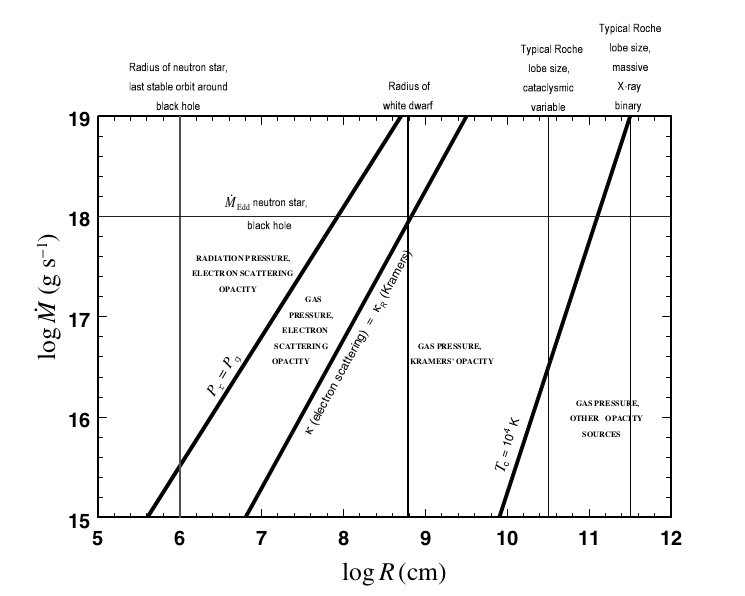
\includegraphics[width=1\linewidth]{MappaPressione}
		\caption{Mappa dei regimi di pressione in un disco stazionario di Shakura e Sunyaev}
		\label{fig:MappaPressione}
	\end{figure}
	
	E' possibile derivare un importante risultato relativo alle regioni dominate da pressione di radiazione relativo all'altezza del disco a partire dal sistema delle equazioni per un disco stazionario.
	
	In particolare dalle formule per $H$, $c_s$, $P$ e $T_c$ e trascurando i termini relativi alla pressione gassosa si trova che la velocità del suono nel disco vale
	\begin{equation*}
		c_s^2=\frac{3GM\dot{M}\tau}{8\pi R^3\rho c}\left[1-\left(\frac{R_{\star}}{R}\right)^{1/2}\right]
	\end{equation*}
	E poiché in queste regioni l'opacità è dovuta allo scattering elettronico, la profondità ottica sarà descritta da
	\begin{equation*}
		\tau=\Sigma\kappa_R(e.s.)\cong\rho H\sigma_T/m_p
	\end{equation*}
	Quindi sostituendo questi risultati nella formula per l'altezza locale si trova che
	\begin{equation}
		H\cong\frac{3\sigma_T\dot{M}}{9\pi m_pc}\left[1-\left(\frac{R_{\star}}{R}\right)^{1/2}\right]
	\end{equation}
		 
	E possiamo dire che l'altezza del disco nelle regioni supportate da pressione di radiazione è circa indipendente dal raggio. Questo è legato al fatto che le forze di pressione $\sim T_c^4\sim M\dot{M}R^{-3}$ sono opposte alla componente verticale della gravità $\propto MHR^{-3}$.
	
	Posso legare questa formula dell'altezza del disco al limite di Eddington
	\begin{equation*}
		\dot{M}=\frac{4\pi GMm_pc^3}{\sigma_T \eta}
	\end{equation*}
	
	Che la fa diventare quindi una condizione sul tasso di accrescimento perché sia mantenuta la struttura sottile del disco
	\begin{equation}
		H\cong\frac{3R_{\star}}{4\eta}\frac{\dot{M}}{\dot{M}_{crit}}\left[1-\left(\frac{R_{\star}}{R}\right)^{1/2}\right]
	\end{equation}
	
	Col loro modello SeS sono stati in grado di dimostrare quindi come l'accrescimento possa produrre una luminosità superiore a quella limite di Eddington, ma hanno anche dedotto che in queste condizioni la pressione radiativa avrebbe espulso la materia in eccesso, cosa che si è osservata accadere  nelle sorgenti x ultra-luminose (ULXs).
	
	Comunque questo non è ovviamente l'unico caso in cui il disco smetta di essere sottile, per esempio anche una temperatura centrale molto superiore di quella di un corpo nero porterebbe a risultati simili.
	
\subsection{Spettro di emissione}
	Abbiamo prescritto che il disco sia otticamente spesso nella direzione $z$, per cui mi aspetto ogni elemento del disco irradi come un corpo nero e quindi con temperatura $T(R)$ tale che
	\begin{equation}
		\sigma T^4(R)=D(R)
	\end{equation}
	
	Da cui ricavo, utilizzando la definizione di $D(R)$
	\begin{equation}
		T(R)=\left\{\frac{3GM\dot{M}}{8\pi R^3\sigma}\left[1-\left(\frac{R_{\star}}{R}\right)^{1/2}\right]\right\}^{1/4}
	\end{equation}
	
	Posso trattare questa temperatura come un valore efficace per il disco, da cui ricavare un valore dell'intensità per frequenza emessa da ogni suo elemento d'area
	\begin{equation}
		I_\nu=B_\nu[T(R)]=\frac{2h\nu^3}{c^2(e^{h\nu/kT(R)}-1)}
	\end{equation}
	
	Questo risultato non tiene conto dell'effetto di redistribuzione dell'intensità rispetto alle frequenze prodotto dall'atmosfera otticamente sottile del disco.

	Il profilo di temperatura efficace del disco ha un andamento radiale $T(R)\propto R^{-3/4}$ indipendente dal meccanismo di trasporto del momento angolare ed è stato confermato negli anni da osservazioni dello spettro di emissione dei dischi e dalla misura della loro luminosità durante delle eclissi.
	
	Per un osservatore il cui angolo di vista abbia un angolo $\theta$ rispetto alla normale al piano del disco, posso definire il flusso per frequenza come
	\begin{equation}
		F_\nu=\frac{2\pi \cos{\theta}}{D^2}\int^{R_{e}}_{R_{\star}}RI_\nu dR=\frac{4\pi h\nu^3\cos{\theta}}{c^2D^2}\int^{R_{e}}_{R_{\star}}\frac{R}{e^{h\nu/kT(R)}-1}dR
	\end{equation}
	
	Con $R_e$ il raggio esterno del disco.
	
	Questo flusso è indipendente dalla viscosità per le ipotesi di corpo nero e disco stazionario.
	
	\begin{figure}[H]
		\centering
		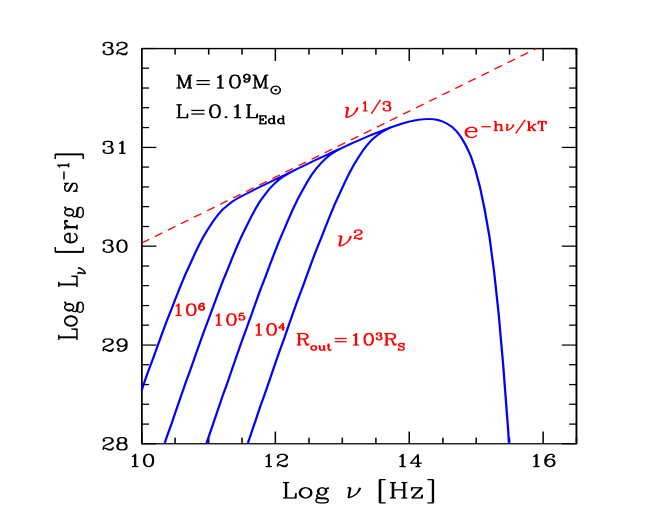
\includegraphics[width=0.7\linewidth]{SpettroDiscoGhisellini}
		\caption{Spettro di un disco di accrescimento nel caso di un buco nero supermassiccio}
		\label{fig:SpettroDiscoGhisellini}
	\end{figure}	

	Se rappresento lo spettro in un sistema bilogaritmico\footnote{Immagine da \cite{GhiselliniRadiativi}} posso apprezzare il comportamento asintotico del flusso, che dipende da quello della plankiana
	\begin{equation}
		F_\nu\propto\begin{cases}
						\nu^2 & \nu\ll kT(R_{e})/h \quad\textit{``regione di Rayleigh-Jeans"}\\
						\nu^{1/3} & kT(R_{\star})/h\ll\nu\ll kT(R_{e})/h\\
						e^{-h\nu/kT} & \nu\gg kT(R_{\star})/h\quad\textit{``regione di Wien"}						
					\end{cases}
	\end{equation}
	Il comportamento a frequenze intermedie $F_\nu\propto\nu^{1/3}$ è considerato caratteristico dei dischi di accrescimento e la lunghezza della regione con quella pendenza dipende dalla differenza di temperatura tra il bordo interno e quello del disco. Se $T(R_{\star})\cong T(R_{e})$ lo spettro di emissione del disco si avvicina sempre più a quello di un corpo nero.
		
\newpage
\section{Evoluzione temporale dei dischi e instabilità}
	Una \textit{soluzione} stazionaria di un sistema si dice \textit{instabile} se, quando viene sottoposta ad una perturbazione, questa continua a crescere invece che diminuire in intensità col tempo.

	Quindi la prima ragione per studiare l'evoluzione temporale del disco è che un'analisi della dipendenza dal tempo dei parametri che lo definiscono ci permette di verificarne la stabilità rispetto a piccole perturbazioni. 
	
	Un disco di accrescimento stazionario deve essere ovviamente stabile. Ogni instabilità derivata dal sistema delle equazioni che lo definiscono deve dipendere da un errore tra le ipotesi con cui è costruito il modello usato per l'accrescimento o quello del disco stazionario stesso. Si potrebbe quindi dire più correttamente che non ci si deve aspettare le instabilità siano reali, ma solo che siano la dimostrazione dell'inconsistenza interna delle ipotesi che si stavano utilizzando.
	
	Una seconda ragione per studiare l'evoluzione delle soluzioni è che, un modello stazionario come quello di Shakura e Sunyaev ha parametri praticamente indipendenti dall'ordine di grandezza dal coefficiente $\alpha$. Le osservazioni di dischi stazionari non possono quindi migliorare la nostra conoscenza della viscosità, mentre la ricerca e lo studio delle instabilità del disco permettono di evidenziare incertezze nel modello e di fare osservazioni quantitative riguardo alla viscosità.
	
	Nonostante la sua eleganza e la semplicità delle ipotesi su cui era costruito, il modello di Shakura e Sunyaev è stato immediatamente riconosciuto dai suoi autori come instabile sotto certe condizioni nell'articolo in cui l'hanno descritto per la prima volta. Pochi mesi dopo la pubblicazione dell'articolo del 1973, sono stati in molti a cercare subito di descrivere le instabilità dei dischi $\alpha$ e a confrontarne le soluzioni con le osservazioni (limitate a pochi oggetti all'epoca e in particolare dirette verso Cygnus X-1) per modificarlo e costruirne una versione stabile e coerente.
	
	\paragraph{Tempi scala del disco}	

	La struttura del disco può variare in diverse scale temporali, a seconda del tipo di fenomeno che la sta interessando. 	
	
	Il primo ad aver costruito un modello dipendente dal tempo di disco di Shakura e Sunyaev è stato Alan Lightman, con i suoi due articoli del 1974 e poi con i suoi lavori firmati anche da Douglas Eardley e Stuart Shapiro sempre del 1974 e poi del 1976 \footnote{\cite{LightmanEardley1974} e \cite{ShapiroLightmanEardley1976}}. 
	
	Lightman ha avuto l'intuizione di analizzare l'evoluzione temporale del disco a partire dallo studio delle relazioni che legano le scale temporali, per caratterizzare diversi tipi di instabilità.	
	
	La più breve scala temporale caratteristica del disco è quella \textit{dinamica}
	\begin{equation}
		t_\phi\sim\frac{R}{v_\phi}\sim\Omega_K^{-1}
	\end{equation}
	Dove si assume che la scala di lunghezze tipica dei gradienti di densità superficiale nel disco è $\sim R$.
	
	Il tempo scala dinamico è caratteristico di ogni disomogeneità del disco, come i flare sulla sua superficie, ma anche dei processi con cui viene stabilito l'equilibrio idrodinamico nella direzione del disco. Infatti si dimostra utilizzando la formula per l'altezza nel disco che
	\begin{equation}
		t_z=\frac{H}{c_s}\sim \frac{R}{c_s}\frac{c_s}{v_\phi}\sim t_\phi
	\end{equation}
	
	I processi legati al trasporto di materia verso il centro del disco avvengono invece nel già citato tempo scala viscoso, che considerando l'assunzione di SeS sulla viscosità diventa
	\begin{equation}
		t_{visc}\sim\frac{R^2}{\nu}\sim\frac{1}{\alpha}\frac{R^2}{Hc_s}=\frac{1}{\alpha}\frac{Rv_\phi}{Hc_s}t_\phi
	\end{equation}

	La scala temporale termica si può definire come il rapporto fra la quantità di calore per unità di volume del disco e la quantità di energia dissipata termicamente, ovvero il tempo necessario a recuperare l'equilibrio termodinamico.
	
	Poiché il calore per unità di superficie del disco è $\sim\rho kT/\mu m_p\sim\rho c_s^2$, vale
	\begin{equation*}
		t_{th}\sim\Sigma c_s^2/D(R)
	\end{equation*}
	
	Che per un disco kepleriano ($\Omega=\Omega_K$), per la definizione di $D(R)$, diventa
	\begin{equation}
		t_{th}\sim\frac{R^3c_s^2}{GM\nu}\sim\frac{c_s^2}{v_\phi^2}t_{visc}
	\end{equation}
	
	Quindi, assumendo $\alpha\lesssim1$ abbiamo che
	\begin{equation}
		t_\phi\sim t_z\lesssim t_{th}\ll t_{visc}	
	\end{equation}

	Questa gerarchia si dimostra essere corretta per un disco ed è un'ulteriore conferma che l'ipotesi che la materia del disco percorra orbite circa kepleriane.

	Tramite il sistema delle equazioni del disco si trova che, per parametri tipici, i tempi scala termico e dinamico sono dell'ordine dei minuti e quello viscoso va dai giorni alle settimane.

	La netta distinzione fra i tempi scala permette di distinguere di conseguenza diversi tipi di perturbazione che può interessare il disco, evidenziandone delle instabilità.
	
\subsection{Instabilità termica}
	
	Si definisce \textit{instabilità termica} quella che dipende da una perturbazione che varia in un arco di tempo dell'ordine di $t_{th}$. Lo sviluppo di questo tipo di instabilità nel modello di SeS è stata prevista la prima volta da Pringle, Rees e Pacholczyck nel loro articolo del 1973\footnote{\cite{PringleReesPacholczyk1973}. L'articolo, scritto dopo la pubblicazione del lavoro dello stesso anno di Shakura e Sunyaev, è concentrato sullo spettro di emissione che ci si aspettava producessero i dischi, confrontato da quello prodotto da un possibile accrescimento sferico, come era inteso da Salpeter. La stabilità termica viene introdotta come una condizione necessaria al disco per irradiare senza "spegnersi".}

	Poiché $t_{th}\ll t_{visc}$ e le variazioni di origine viscosa sono legate a variazioni della densità superficiale del disco, si può approssimare $\Sigma\sim cost$ durante il tempo di crescita della perturbazione termica e considerare solo l'evoluzione dello spessore del disco $H$ o equivalentemente della sua temperatura centrale in funzione del raggio $T_c(R)$.
	
	Nell'ipotesi in cui $\alpha<1$, vale inoltre $t_{th}>t_\phi\sim t_z$. In questo caso la struttura verticale del disco risponderà abbastanza velocemente ai cambiamenti dovuti all'instabilità termica da rimanere sempre approssimativamente in equilibrio idrodinamico. La formula dell'altezza del disco durante la crescita di un'instabilità termica deve avere quindi una forma del tipo: $H\sim c_s(T_s)\left(\frac{R^3}{GM}\right)^{1/2}$.
	
	Nel disco l'equilibrio termodinamico corrisponde alla condizione per cui sono uguali il tasso di raffreddamento locale del disco $Q^-$ ($erg\,s^{-1}\,cm^{-3}$) e quello di riscaldamento dovuto alla dissipazione viscosa $Q^+\sim D/H$. In particolare il tasso di raffreddamento può avere forme diverse o dipendere da molti fattori insieme, oltre all'emissività del disco, ma nel caso di $\Sigma$ fissata e la direzione $z$ in equilibrio idrostatico, si possono esprimere $Q^+$ e $Q^-$ come funzioni della sola $T_c$. 
	
	Se un piccolo aumento della temperatura centrale del disco $dT_c$ fosse sufficiente a far crescere $Q^+$ più velocemente di $Q^-$, questo romperebbe l'equilibrio e la temperatura centrale dovrebbe continuare a crescere, troppo poco supportata da un raffreddamento sempre meno adeguato, portando quindi alla rottura della struttura del disco, che potrebbe formare una nube geometricamente spessa o disperdersi. Non è per nulla banale capire quale delle due evoluzioni possa capitare ad un sistema, poiché il processo dipende molto dalla regione in cui si crea l'instabilità.
	
	In generale si può quindi scrivere la \textit{condizione di instabilità termica}\footnote{Pringle 1977} come
	\begin{equation}
		\frac{dQ^-}{dT_c}<\frac{dQ^+}{dT_c}
	\end{equation}

	\paragraph{Regioni otticamente sottili}
	Una regione del disco attraversata da una perturbazione può risultare così poco densa che la profondità ottica lungo la direzione verticale sia $\tau\ll1$. In questo caso ha senso supporre che il tasso di raffreddamento $Q^-$ dipenderà solo dall'emissività, che per una regione otticamente sottile vale $4\pi j(\rho,T_c)$. In particolare questo tipo di gas emette con processi a due corpi, tali per cui vale $4\pi j\propto \rho^2\Lambda(T_c)$. 
	
	La \textit{curva di raffreddamento} $\Lambda$ dipende dall'equilibrio di ionizzazione mantenuto nel gas (se per fotoionizzazzione, scattering o altri processi) ed è la sua forma funzionale rispetto a $T_c$ a determinare se l'instabilità cresca o no nel disco.
	
	Durante la perturbazione, deve valere nelle zone dominate dalla pressione del gas
	\begin{align*}
		Q^-&=4\pi j\propto\rho^2\Lambda\sim\left(\frac{\Sigma}{H}\right)^2\Lambda\sim c_s^{-2}\Lambda\sim T_c^{-1}\Lambda\\
		Q^+&\sim\frac{D}{H}\sim\frac{\nu}{H}\sim\alpha c_s\sim\alpha T_c^{1/2}
	\end{align*}
	
	Quindi il criterio di instabilità termica è che $\Lambda/\alpha$ cresca più lentamente di $T_c^{3/2}$, ovvero quando
	\begin{equation}
		\frac{d\ln{(\Lambda/\alpha)}}{d\ln{T_c}}<\frac{3}{2}
	\end{equation}
	
	Si dimostra che la forma funzionale di $\Lambda$ è circa la stessa, indipendentemente dallo spessore ottico o se la pressione è dominata dal termine radiativo piuttosto che da quello gassoso. Quindi per $\alpha\sim cost$, $\Lambda(T_c)$ decresce per $T_c\gtrsim10^4\,K$ e mi aspetto le regioni otticamente sottili del disco siano termicamente instabili proprio al di sopra di questi valori della temperatura centrale\footnote{E' importante sottolineare comunque come $\Lambda$ dipenda dalla nostra condizione su $\alpha$: se per esempio, invece dell'assunzione di Shakura e Sunyaev ipotizzassimo che $\alpha\sim T^{-2}_c$ ci dovremmo aspettare che l'instabilità si estenda nelle regioni con $T_c\lesssim10^4\,K$. Comunque questo non è plausibile in quanto ci aspettiamo $\alpha\lesssim1$ ovunque sul disco e un risultato tipo $\alpha\sim T^{-2}_c$ non potrebbe valere per un intervallo di temperature troppo ampio.}.
		
	\paragraph{Regioni otticamente spesse}
	Nel caso di una regione otticamente spessa invece, si dimostra che il tasso di raffreddamento vale, tenendo conto anche il riassorbimento locale di energia irradiata e utilizzando l'opacità di Kramer:
	\begin{equation}
		Q^-=\frac{dF}{dz}\sim\frac{\sigma T_c^4}{\kappa_R\rho H^2}\sim\frac{T_c^{15/2}}{\Sigma^2}\sim T_c^{15/2}
	\end{equation}
	
	Inoltre perché nelle regioni dominate da pressione gassosa vale $Q^+\sim \alpha T_c^{1/2}$, le regioni otticamente spesse sono termicamente stabili a meno che $\alpha$ non decresca più velocemente di $T_c^{-7}$.
	
	Si dimostra che le condizioni di stabilità per queste zone opache è simile nel caso si trovino in regioni dominate dalla pressione radiativa o nel caso seguano altre formule per l'opacità.

\subsection{Instabilità viscosa}
	I cambiamenti nella struttura del disco che avvengono nel tempo scala viscoso includono le instabilità viscose e l'evoluzione del disco a seguito di un cambiamento delle condizioni ambientali.
	
	Poiché $t_{visc}\gg t_{th}\gtrsim t_z$, mi aspetto che il disco mantenga durante questo tipo di cambiamento, l'equilibrio termodinamico e quello idrodinamico. Posso quindi assumere che $Q^+=Q^-$ e che la viscosità ad un raggio fissato sia definita come funzione della sola densità superficiale $\Sigma$. 
	
	Sotto queste ipotesi mi aspetto che le molte equazioni valide per il modello di disco stazionario debbano rimanere valide anche per il modello dipendente dal tempo. 
	
	\paragraph{Evoluzione temporale del disco}
	In particolare, a cambiare sono l'equazione del trasporto radiativo (numero 5 nel sistema precedente), in cui si deve utilizzare la definizione di $D(R)$ derivata studiando le forze viscose nel disco:
	\begin{equation}
		\frac{4\sigma}{3\tau}T_c^4=\frac{9}{8}\nu\Sigma\frac{GM}{R^3}
	\end{equation}
	e l'equazione numero 7, derivata come integrale delle conservazioni della massa e del momento, che si deve sostituire con l'equazione di evoluzione $\partial \Sigma/\partial t$, ponendo $\dot{M}=2\pi R\Sigma(-v_R)$ e che quindi diventa
	\begin{equation}
		2\pi R\frac{\partial \Sigma}{\partial t}=\frac{\partial\dot{M}}{\partial R}
	\end{equation}
	Il sistema delle soluzioni di un sistema che varia nel tempo è quindi
	\begin{equation}
	\begin{cases}
		1.\quad \rho=\Sigma/H\\
		2.\quad H=c_sR^{3/2}/(GM)^{1/2}\\
		3.\quad c_s^2=P/\rho\\
		4.\quad P=\frac{\rho\kappa T_c}{\mu m_p}+\frac{4\sigma}{3c}T_c^4\\
		5.\quad \frac{4\sigma}{3\tau}T_c^4=\frac{9}{8}\nu\Sigma\frac{GM}{R^3}\\
		6.\quad \tau=\rho H\kappa_R(\rho,T_c)=\tau(\Sigma,\rho,T_c)\\
		7.\quad 2\pi R\frac{\partial \Sigma}{\partial t}=\frac{\partial\dot{M}}{\partial R}\\
		8.\quad \nu=\nu(\rho,T_c,\Sigma,\alpha,...)		
	\end{cases}
	\end{equation}
	
	Questo è di nuovo un sistema di otto equazioni per otto incognite $\rho$, $\Sigma$, $H$, $c_s$, $P$, $T_c$, $\tau$ e $\nu$, funzioni di $R$, $t$ e di un parametro nella prescrizione sulla viscosità ($\alpha$) dell'equazione 8. 
	
	Imposte delle condizioni al contorno per l'equazione di diffusione (la numero 7), il sistema si può risolvere e permette di ricavare anche le equazioni per $\dot{M}$ e $v_R$.
	
	Poiché la dipendenza dal tempo è presente solo nella settimana equazione, posso provare a esprimere le altre grandezze in funzione della densità superficiale, poiché in questa forma dipendono da $t$ solo implicitamente.
	
	Con delle operazioni algebriche sulle equazioni da 1 a 6 trovo
	\begin{gather}
		\frac{GM\Sigma H}{R^3}=\frac{\kappa T_c\Sigma}{\mu m_p H}+\frac{4\sigma}{3c}T_c^4\\
		T^4_c=\frac{27}{32\sigma}\Sigma^2\kappa_R\nu\frac{GM}{R^3}
	\end{gather}
	
	Poiché $\kappa_R$ e $\nu$ sono in generale funzioni di $\Sigma/H$, $T_c$ e $R$, posso decidere di eliminare $\kappa_R$ e $\nu$ dal sistema scrivendo le altre grandezza in funzione dei soli $R$ e $\Sigma$.
		
	\paragraph{Instabilità viscosa}
	
	Nel caso in cui l'opacità sia descritta efficacemente dalla legge di Kramer e vale l'assunzione di Shakura e Sunyaev sulla viscosità, l'equazione per la temperatura centrale diventa
	\begin{equation*}
		T^4_c\propto\alpha\Sigma^3HT_c^{-7/2}\left(\frac{GM}{R^3}\right)^{3/2}
	\end{equation*}
	
	Sostituendo questo risultato nelle equazioni del sistema della struttura del disco, si ricava una funzione per il coefficiente di viscosità in funzione solo di $R$ e $\Sigma$
	\begin{equation*}
		\nu=\alpha c_sH=\alpha H\left(\frac{\kappa T_c}{\mu m_p}\right)^{1/2}=\nu(R,\Sigma)
	\end{equation*}
	
	E con questa condizione abbiamo già osservato che l'equazione 7 diventa un'equazione non lineare di diffusione per $\Sigma(R,t)$\footnote{Questa condizione non sarebbe rispettata se per esempio $\alpha$ non fosse una funzione delle condizioni locali del disco, ma definita da fattori ambientali. In quel caso avrebbe potuto avere anche una dipendenza esplicita dal tempo. Questo tipo di ipotesi è stata considerata nella costruzione di modelli alternativi a quello di disco sottile o a due temperature.}. L'equazione è così risolvibile numericamente e permette di ricavare la soluzione completa in funzione del tempo.

	Per studiare efficacemente gli effetti delle instabilità viscose, si può decidere di perturbare la densità superficiale del disco con una variazione a simmetria assiale rispetto al BH (e che quindi agisce coerentemente ad ogni raggio).
	
	Se $\Sigma_0$ è la densità superficiale per il disco stazionario e $\delta\Sigma$ la sua variazione, posso descriverne l'evoluzione come
	\begin{equation}
		\Sigma(R,t)=\Sigma_0(R)+\delta\Sigma(R,t)
	\end{equation}
	
	Con la sostituzione $\mu(R,\Sigma,t)\equiv\nu(R,\Sigma,t)\Sigma(R,t)$, si può dimostrare che $\delta\mu=\frac{\partial\mu}{\partial\Sigma}$ e quindi che la perturbazione viscosa è regolata dalla legge
	\begin{equation}
		\frac{\partial}{\partial t}(\delta\mu)=\frac{\partial\mu}{\partial\Sigma}\frac{3}{R}\frac{\partial}{\partial R}\left[R^{1/2}\frac{\partial}{\partial R}(R^{1/2}\delta\mu)\right]
	\end{equation}
	
	Questa è un'altra equazione differenziale, ma si distingue da quella di $\Sigma$ per la particolarità di essere proporzionale al termine $\frac{\partial\mu}{\partial\Sigma}$, che in linea di principio non posso dire sia negativo o positivo.
	
	Se $\partial\mu/\partial\Sigma>0$, mi aspetto di trovare una soluzione all'equazione differenziale simile a quella per il caso del disco stazionario, per cui la perturbazione si estingue in circa $t_{visc}$ e la diffusione della materia del disco prosegue verso il BH, trasportando momento angolare verso l'esterno. 
	
	Al contrario, se $\partial\mu/\partial\Sigma<0$, quello che succede è che più materia sarà accresciuta verso le regioni del disco localmente più dense e materiale sarà estratto da quelle meno dense. Questo porta il disco alla formazione di anelli di materia e interrompe il processo di accrescimento al corpo massiccio centrale.
	
	Posso quindi dire che il segno di $\partial\mu/\partial\Sigma$ costituisce una \textit{condizione di instabilità viscosa} per il disco.
	
	\paragraph{Significato fisico della condizione}
	Le soluzioni dell'equazione di diffusione di $\mu$ si possono decifrare meglio osservando che per un disco stazionario valgono
	\begin{gather*}
				T^4(R)=\frac{3GM\dot{M}}{8\pi R^3\sigma}\left[1-\left(\frac{R_{\star}}{R}\right)^{1/2}\right]\\
				\nu\Sigma=\frac{\dot{M}}{3\pi}\left[1-\left(\frac{R_{\star}}{R}\right)^{1/2}\right]
	\end{gather*}
	E quindi, se considero $\dot{M}$ e $T(R)$ come i valori di equilibrio di tasso di accrescimento e temperatura superficiale del disco, posso scrivere che ad ogni istante $\mu=\nu\Sigma\propto\dot{M}\propto T^4(R)$.
	
	Posso allora riscrivere il criterio di instabilità equivalentemente come
	
	\begin{align*}
		\frac{\partial\dot{M}(R)}{\partial\Sigma}&<0 \\
		\textit{oppure} \\
		\frac{\partial T(R)}{\partial\Sigma}&<0
	\end{align*}
	
	Questo significa esattamente che in un disco instabile il tasso di accrescimento cresce nelle regioni in cui diminuisce la densità superficiale e quindi la materia viene estratta per venire trasportata verso le regioni più dense. Inoltre le regioni localmente meno dense cresceranno più velocemente delle altre.
	
	La condizione sulla temperatura superficiale invece significa che, se nelle regioni viscosamente stabili ($\partial T(R)/\partial\Sigma>0$) ogni piccola variazione della densità superficiale comporta una piccola variazione della temperatura superficiale e quindi un ritorno all'equilibrio in un tempo scala termico locale, nelle regioni viscosamente instabili piccole variazioni della densità superficiale possono provocare grandi variazioni della temperatura. Questo perché si può notare dai diagrammi $T-\Sigma$ che il riscaldamento domina sul raffreddamento a destra dell'equilibrio, inteso come soluzione stazionaria\footnote{Immagine da \cite{FrankKingRaineAccretionPower}}.	
	
	\begin{figure}[H]
		\centering
		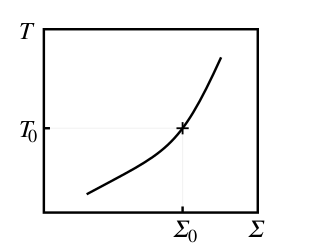
\includegraphics[width=0.4\linewidth]{TemperaturaDensita}
		\caption{Diagrammi $T-\Sigma$ di sistemi con una sola soluzione stazionaria $(T_0,\Sigma_0)$}
		\label{fig:TemperaturaDensita}
	\end{figure}
	
	Queste due interpretazioni fisiche della condizione di instabilità viscosa del disco del disco sono state proposte separatamente e si devono a Lightman ed Eardley\footnote{\cite{LightmanEardley1974}} e a Shakura e Sunyaev\footnote{\cite{ShakuraSunyaev1976}}.

\newpage
\section{Evidenze dell'instabilità del modello di Shakura e Sunyaev}
	Con i suoi articoli seminali sull'evoluzione temporale del modello di Shakura e Sunyaev, Lightman è riuscito a osservare e criticizzare per primo diversi problemi insiti nell'ipotesi $\alpha$ sulla viscosità dei due scienziati moscoviti, aprendo la strada per una lunga serie analisi riguardo la stabilità del modello e alla ricerca di una descrizione consistente e valida dei processi di accrescimento.
	
	\subsection{Instabilità e collasso del disco nelle regioni dominate da pressione di radiazione}
	Tanto per cominciare, è possibile dimostrare che nelle regioni centrali del disco secondo SeS sono contemporaneamente viscosamente e termicamente instabili\footnote{Immagine da \cite{ShakuraSunyaev1973}}.
	
	\begin{figure}[H]
		\centering
		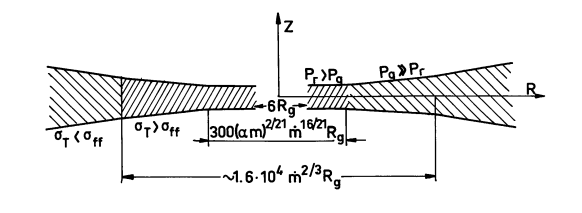
\includegraphics[width=0.9\linewidth]{RegioniDisco}
		\caption{Rappresentazione delle diverse regioni del disco secondo Shakura e Sunyaev, distinte in base alle loro condizioni fisiche}
		\label{fig:RegioniDisco}
	\end{figure}
	
	Gli $\alpha$ dischi sono instabili ad alti tassi di accrescimento sub-critici a raggi brevi per via del drastico aumento di temperatura nella regione in cui la pressione passa dall'essere dominata dalla componente gassosa a quella in cui è dominata dalla componente radiativa. In queste regioni un piccolo aumento della temperatura comporta un aumento importante della pressione e quindi del riscaldamento, poiché $G\propto\alpha P$. Questo comporta un aumento della temperatura che non è bilanciato da nessuna diminuzione dell'opacità e che quindi provoca una dispersione di calore enorme.
	 
	Questa instabilità del modello è un campanello d'allarme sulla validità dell'assunzione $\alpha$, poiché l'analisi della struttura del disco a regimi sub-critici e un grande numero di osservazioni ci dicono che più della metà dell'emissione dovuta all'accrescimento avviene proprio nelle regioni più interne al disco.
	
	L'istabilità termica nel disco porta all'instaurarsi di un'instabilità viscosa, poiché l'aumento di temperatura comporta un aumento del tasso di accrescimento attraverso ogni anello che lo costituisce. Ad ogni raggio termicamente instabile $\dot{M}$ può quindi crescere fino a superare il tasso di materia in ingresso dai raggi più esterni del disco. In questa situazione il materiale viene quindi raccolto intorno al raggio dell'anello, provocando un'aumento della pressione locale e il suo riscaldamento. La temperatura inizia però a diminuire con il rallentamento di questo processo di disgregazione, fino a portare l'anello a temperature abbastanza basse da riddure il tasso di accrescimento nell'anello abbastanza da renderlo minore di quello della materia in ingresso, permettendo al disco di riformarsi e riattivando l'instabilità termica, in una situazione detta di \textit{ciclo limite}\footnote{Immagine da \cite{DoneGierlinskiKubota2007}}.

	\begin{figure}[H]
		\centering
		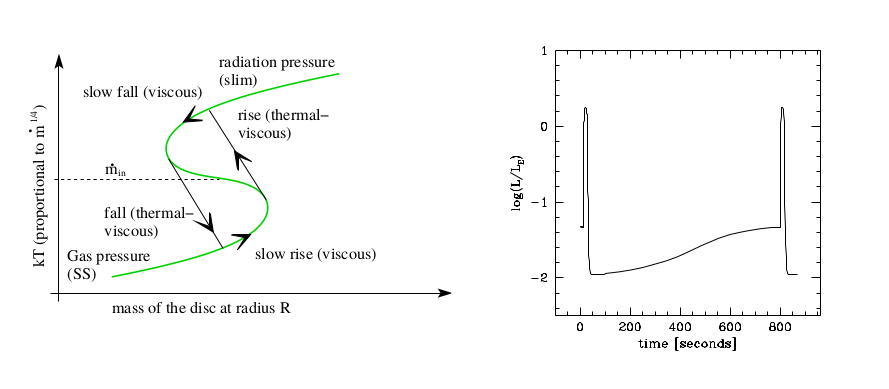
\includegraphics[width=0.9\linewidth]{PresInstLimitCycle}
		\caption{Il grafico a sinistra mostra l'effetto locale dell'instabilità, con il tasso di accrescimento che varia discontinuamente ad un raggio fissato. I prolungamenti del grafico mostrano le situazioni descritte da Shakura e Sunyaev, con le regioni interne dominate dalla pressione di radiazione e quella del cosiddetto \textit{slim disc model} dove è invece la pressione gassosa a  dominare nelle stesse regioni. Il diagramma a destra mostra il risultato di una computazione dell'effetto di questa instabilità sulla luminosità di un $\alpha$ disco con $\alpha=0.01$ e $L/L_{Edd}=0.06$. Nessun sistema binario contenente buchi neri osservato finora ha un comportamento simile.}
		\label{fig:PresInstLimitCycle}
	\end{figure}
	
	Finora comunque non sono trovate prove che dimostrino l'esistenza dell'instabilità nelle regioni dominate da pressione di radiazione prevista dal modello di SeS. Dischi descritti con la prescrizione di $\alpha$ dovrebbero diventare instabili a $L\lesssim L_{edd}$, producendo cicli limite\footnote{L'unica quasi eccezione è la binaria super-critica GRS 1915+105, che mostra qualcosa di simile a un ciclo limite}. 
	
	Quello che sembra più logico fare, per superare questo tipo di instabilità è cambiare la condizione sulla viscosità, di per sé completamente ad hoc, ma non è ancora stata trovata una soluzione che che fosse coerente con tutte le osservazioni e non si potesse giustificare fisicamente\footnote{Come spiegato in \cite{Pringle1981}}. Comunque si sono trovate prescrizioni diverse a quella di Shakura e Sunyaev sul momento torcente analiticamente stabili ovunque\footnote{Stella e Rosner 1984}. 
		
	\paragraph{L'effetto di avvezione e convezione}

	Per gli $\alpha$ dischi non esiste una soluzione stabile ad alto tasso di accrescimento e alte temperature e il modello prevede la distruzione dell'intero disco.
	
	Un modo per aggirare questa difficoltà è includere un meccanismo di avvezione o convezione radiali nelle equazioni del sistema per le regioni interne del disco, che non erano considerato nella soluzione standard di Shakura e Sunyaev. Questo tipo di processo fornirebbe un ulteriore meccanismo di raffreddamento per le regioni interne del sistema oltre all'irraggiamento, poiché parti dell'energia verrebbero trasportate con la materia nel disco. 
		
	Bisogna osservare però come il disco avrebbe $H/R\sim1$ nelle regione dominata da avvezione o convezione e quindi i tempi scala viscoso e termico sarebbero localmente circa uguali, comportando che la quantità di materiale negli anelli varierebbe anche con la temperatura. Inoltre l'ipotesi di un disco che includa l'avvezione o la convezione radiale non cambierebbe in alcun modo il meccanismo viscoso. 
	
	Questi due effetti insieme implicano che l'instabilità locale possa propagarsi in un disco soggetto ad avvezione, ma solo nella regione dominata da pressione di radiazione che diventerebbe globalmente instabile, invece di tutto il disco come prevede il modello di Shakura e Sunyaev.
	
		Attualmente, si sta vagliando l'ipotesi che il momento torcente effettivo nel disco scali rispetto alla temperatura più di quanto previsto dalla pressione di radiazione, ma meno di quanto previsto dalla sola pressione gassosa. Analisi numeriche del momento esercitato dalla MRI suggeriscono che il riscaldamento sia proporzionale alla media geometrica e alla pressione totale del gas (Merloni 2003). Questo tipo di disco sarebbe instabile a $\sim 0.3L_{edd}$, ma l'effetto del trasporto di materia per mezzo di avvezione o convezione tra anelli vicini comporterebbe che il disco assuma un profilo smorzato (\textit{damped out}), rendendo la prescrizione stabile a luminosità più alte $\sim 0.4L_{edd}$ (Honma e Matsumoto 1991, Merloni e Nayakshin 2006). 
	
	Questa ipotesi è promettente in quanto la struttura di un disco di questo tipo sarebbe molto sensibile a piccole variazioni dell'effettiva prescrizione sull'$\alpha$. Quindi una piccola variazione nel modo in cui la tensione scala rispetto alla media geometrica potrebbe restituire il limite osservato per la luminosità di $L/L_{Edd}\sim0.5$ e potrebbe anche giustificare l'instaurarsi dell'instabilità di pressione a luminosità superiori, spiegando il ciclo limite osservato in GRS 1915+105, l'unico sistema binario contenente buchi neri nella via lattea che spende un tempo significativo vicino al limite di Eddington. Questa variabilità potrebbe essere collegata al suo essere l'unica sorgente con luminosità sufficientemente alta da instaurare l'instabilità di pressione.
		 
	\paragraph{Dinamica del collasso delle regioni interne del disco}
	
	In un loro articolo del 2004\footnote{\cite{TeresiMolteniToscano2004}}, V. Teresi, D. Molteni ed E. Toscano si sono occupati di studiare l'evoluzione di un disco secondo Shakura e Sunyaev a regime di accrescimento sub-critico, concentrandosi sulle regioni dominate da pressione di radiazione per cercare prove di come potrebbe evolversi, se collassando in una nube otticamente sottile e geometricamente spessa o espandendosi e perdendo materiale fino a smettere di irradiare. 
	
	Questo tipo di simulazione era stato già fatto diverse volte tra gli anni '80 e i primi anni 2000, con risultati discordanti: Taam e Lin\footnote{\cite{TaamLin1984}} hanno osservato delle fluttuazioni nella luminosità del disco legate ad esplosioni o flare, Eggum ha esposto in un suo articolo del 1987 come dai suoi risultati sembrasse il disco fosse destinato ad appiattirsi ed espandersi fino a spegnersi e Fujita e Okuda nel 1998 sembravano aver dimostrato che il disco era effettivamente stabile termicamente a regimi sub-critici di accrescimento nelle regioni dominate da pressione di radiazione, come previsto dal modello di "accrescimento sottile" (\textit{slim accretion model})\footnote{Un modello secondo cui l'instabilità in queste regioni è prevenuta dalla dominanza del flusso di calore avvettivo rispetto a quello di calore radiativo verticale}. Il difetto di tutte queste simulazioni era che, con i mezzi disponibili all'epoca in cui sono state fatte, potevano essere solo bidimensionali e l'evoluzione del disco era calcolata per periodi di tempo molto più brevi del tempo scala viscoso. Quindi potevano star descrivendo situazioni transienti e non risvolti definitivi.
	
	I tre italiani, riprendendo un lavoro di Agol del 2001, hanno quindi utilizzato tempi di integrazione più lunghi, riuscendo ad osservare l'effettivo collasso delle regioni interne del disco, che inizia con una serie di fluttuazioni e di instabilità legata a flare e ad un momentaneo recupero della sua luminosità iniziale da parte del disco, che dura appunto meno del tempo scala viscoso.
	
	In particolare hanno osservato come, nonostante il modello di Shakura e Sunyaev non consideri l'eventualità che ci sia un moto convettivo o advettivo radiale nel disco, questo però compare spontaneamente nelle loro simulazioni\footnote{Immagine da \cite{TeresiMolteniToscano2004}}.

	\begin{figure}[H]
		\centering
		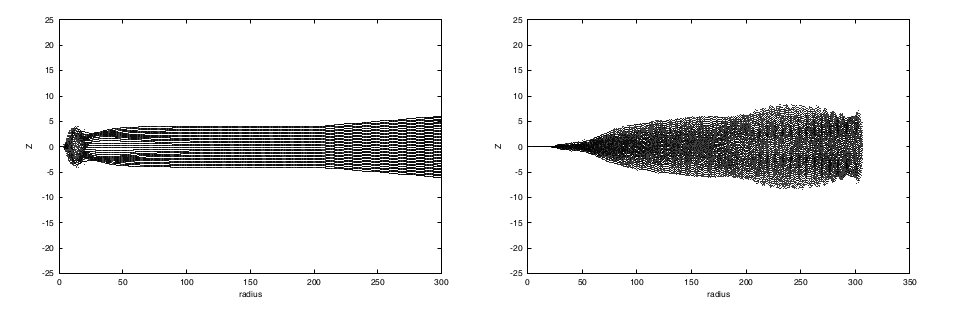
\includegraphics[width=1\linewidth]{CollassoDisco1}
		\caption{Evoluzione del disco con $\alpha=0.01$, $\dot{M}=0.7$, dominio $R_1-R_2=3-300\,h$, $h=0.3$. Nella figura di sinistra viene mostrato a $t=282$ ed è evidente come nei pressi del buco nero centrale ci sia una regione interessata da moti convettivi. La seconda è a $t=12000$ e mostra l'evidente collasso della regione centrale del disco. Le lunghezze sono rappresentate in unità di $R_\star$ e in tempi in unità del periodo orbitale del sistema}
		\label{fig:CollassoDisco1}
	\end{figure}

	\begin{figure}[H]
		\centering
		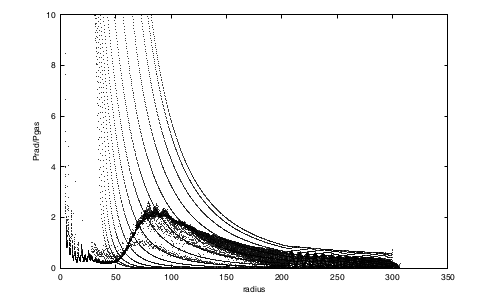
\includegraphics[width=0.8\linewidth]{CollassoDisco2}
		\caption{Diagramma del rapporto tra pressione radiativa e gassosa $P_r/P_g$. A $t=282$ il disco sembra essere dominato da pressione di radiazione fino a $\sim150\,R_\star$, mentre a $t=12000$ è evidente come le sue regioni interne siano collassate e sia dominato da pressione gassosa fino a $\sim70\,R_\star$. Le lunghezze sono in unità di $R_\star$ e in tempi in unità del periodo orbitale del sistema}
		\label{fig:CollassoDisco2}
	\end{figure}
	
	\subsection{Spettro nella banda dei raggi X e Cyg X-1}
	 
	Un sistema in accrescimento che sia stazionario è definito da soli tre parametri, ovvero massa e velocità di rotazione del buco nero e tasso di accrescimento, che possono ridursi a due, studiando sistemi che emettono alla stessa frazione della luminosità di Eddington e quindi con un simile tasso di accrescimento. Gli unici altri parametri che possono influenzare l'aspetto osservativo dei sistemi sono il loro angolo di inclinazione rispetto alla nostra linea di vista e qualsiasi effetto non stazionario legato alla possibile variabilità della struttura del disco.
	
	La massa del buco nero e la sua inclinazione sono potenzialmente osservabili dall'orbita del sistema binario.
	
	La sua rotazione è più difficile da misurare, ma non avendo effetto sulle regioni oltre l'ultima orbita stabile, mi sono preso la libertà di non considerarlo finora per l'analisi del modello classico di Shakura e Sunyaev.
	
	Neanche il tasso di accrescimento è osservabile direttamente, perché la luminosità per unità di massa si dimostra dipendere dal potenziale gravitazionale del buco nero, che dipende a sua volta dalla sua rotazione e ad effetti relativistici che possono avvenire nella regione tra l'orizzonte del buco nero e l'ISCO.
	
	La luminosità negli X è dunque solo una traccia, probabilmente non lineare, del tasso di accrescimento totale dei sistemi binari con buchi neri.

	Le osservazioni per lunghi periodi degli spettri e delle curve di luce nella banda dei raggi X di sistemi binari, con la loro evidente e rapida variabilità e anche il comportamento legato ai getti che può emettere un disco, si considerano oggi coerenti ad un modello di disco in cui si possono distinguere una regione esterna con struttura da disco $\alpha$, troncata ad un raggio minimo a cui viene sostituita da una regione interna più calda, che sarebbe anche il punto da cui sorgono i getti ("\textit{jet}"). Questo modello è figlio del primo prototipo del cosiddetto \textit{disco a due temperature}, immaginato e descritto da Shapiro, Lightman ed Eardley nel loro articolo del 1976\footnote{\cite{ShapiroLightmanEardley1976}}.
	
	In particolare si osserva che per un raggio di troncamento della regione esterna del disco decrescente, i sistemi sono soliti presentare spettri più morbidi, con frequenze maggiori nello spettro caratterizzato da una legge di potenza e getti più veloci.
	
	Nel loro articolo di review sulle osservazioni svolte fino al 2003 da satelliti X come l'RXTE o il \textit{Ginga} e da satelliti radio, Done, Gierlinksi e Kubota si sono occupati anche di commentare e criticare modelli alternativi a quelli del tipo a due temperature, mostrando come nessuno sia davvero esaustivo nel descrivere la varietà di spettri che si sono osservati emettere i sistemi binari.
	
	Le osservazioni radio sono state fondamentale per collegare definitivamente alla formazione di getti di materia i sistemi in accrescimento, poiché non sono previsti dai modelli standard di accrescimento anche oltre quello di Shakura e Sunyaev.

	Quello che si sta facendo ora è provare a costruire modelli della natura instabile e mutevole della materia in accrescimento per giustificare le osservazioni che si sono fatte.	
	
	Dopo il collasso del flusso caldo interno, lo spettro dei sistemi contenenti un buco nero può risultare dominato dall'emissione del disco. Il suo comportamento è coerente all'esistenza di un'ultima orbita stabile interna e i dati a riguardo permettono anche di calcolare la rotazione del buco nero.
	
	Ad alte luminosità questo tipo di sistema può mostrare una grande varietà di spettri, in cui il disco è deformato dalla comptonizzazione. La struttura del flusso di materia in accrescimento risulta sempre più incerto e turbolento all'avvicinarsi della luminosità al limite di Eddington, con la possibilità che si formino dei venti di materia intensi.

\paragraph{Cyg X-1 e il modello a disco troncato}

Che gli spettri osservati variano drasticamente in forma è un fatto risaputo dalle prime osservazioni in X, in particolare per quanto riguarda il primo oggetto studiato approfonditamente: Cyg X-1, che presenta due spettri molto diversi.

	\begin{figure}[H]
		\centering
		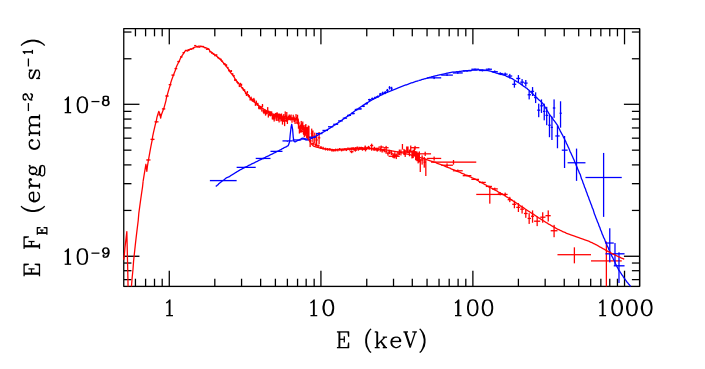
\includegraphics[width=0.8\linewidth]{CygX1}
		\caption{Spettro di Cygnus X-1 in banda X e $\gamma$. Lo spettro morbido è tracciato in rosso e quello duro in blu. L'asse verticale è in unità di $\nu F\nu$, quindi il picco indica l'energia caratteristica dei fotoni in output alla sorgente. Immagine da Gierlinski e al. 1999.}
		\label{fig:CygX1}
	\end{figure}
	
Lo stato "alto" dello spettro è caratterizzato da una componente "morbida" sotto ai $\sim10\,keV$, accompagnata da una complessa coda di emissione non termica dai $500\,keV$ ed oltre\footnote{Gierlinski et al.1999, McConnel et al. 2000}. Questa componente morbida è interpretata come un emissione termica da un disco di accrescimento otticamente spesso intorno al buco nero, riproducibile con un modello di disco multicolore \footnote{Dotani et al. 1997 usando il modello DISKBB. Mitsuba et al. 1984}, che approssima lo spettro di un disco di SeS. Comunque la coda di emissione oltre lo spettro del disco che si estende ad alte energie è inspiegabile utilizzando solo il modello standard di disco.

La discrepanza tra le osservazioni e le previsioni del disco sono anche più marcate sull'altra forma spettrale vista su Cyg X-1, dove una larga frazione della potenza è emessa in uno spettro che non somiglia per niente a quello di un disco. Questi spettri sono chiamati "bassi" o "duri", con picco a $\sim100\,keV$, con una componente di temperatura del disco bassa.

I due spettri insieme richiedono che ci siano due componenti distinte dell'emissione dal sistema in accrescimento. In generale ci sono tracce di una regione otticamente spessa, che può essere dominante (come nel caso della regione morbida), che richiede che parte dell'energia dell'accrescimento sia dissipata in una regione di materiale otticamente sottile, così che l'energia non termalizzi con la temperatura del disco.

	Una possibilità molto promettente per giustificare l'origine della componente otticamente sottile dell'emissione è che sia proprio il disco a diventare otticamente sottile. Perché l'energia del disco si possa termalizzare è fondamentale che il suo spettro sia prodotto da numerosi collisioni tra protoni ed elettroni e tra elettroni e fotoni\footnote{Questo non è sempre vero. Ad esempio nel caso di bassi tassi di accrescimento, per cui anche la densità diventa bassa e non sono possibili gli urti}. Se il disco è abbastanza caldo, diventa più facilmente otticamente sottile alle collisioni tra elettroni e fotoni e quindi deve diventarlo pure per quelle tra protoni ed elettroni. 
	
	Questo fatto è rilevante in quanto i protoni acquistano la parte maggiore dell'energia gravitazionale, ma gli elettroni restano comunque i migliori irradiatori. Una termalizzazione incompleta degli elettroni con i protoni porta alla formazione di un plasma a due temperature, in cui i protoni acquistano molta energia gravitazionale, ma ne cedono poca agli elettroni via urti, mentre gli elettroni acquistano poca energia tramite l'interazione coulombiana, ma ne emettono la maggior parte.
	
	Poiché il flusso sarebbe otticamente sottile, la radiazione sarebbe emessa sotto una forma simile a quella di comptonizzazione, bremsstrahlung e/o ciclo-sincrotrone, piuttosto che quella di corpo nero.
	
	In questo tipo di situazione, la temperatura dei protoni arriverebbe ad essere prossima a quella viriale e quindi il flusso disordinato in accrescimento dovrebbe avere una grande altezza scala $H$, tale per cui le forze di pressione, insieme a quelle centrifughe, sarebbero importanti per bilanciare quella di gravità.
	
	\paragraph{Sviluppi moderni}
	
	Nel dettaglio, la stabilità di questo tipo di struttura calda, otticamente sottile e geometricamente spessa dipende fortemente dalle condizioni che si assumono. Nel loro articolo del 1976, Shapiro Lightman ed Eardley hanno descritto le proprietà del modello a due temperature nel caso in cui non sia presente avvezione, ma è stato dimostrato in alcuni lavori successivi (Ichimaru 1977, Ion Torus: Rees et al. 1982, Advection Dominated Accretion Flow ADAF: Narayan e Yi 1995) come l'avvezione di energia gravitazionale da parte dei protoni dovrebbe sempre essere molto intensa in questo tipo di sistema a due temperature\footnote{ADAF: un modello auto-similare che impone un valore unico per la frazione che subisce avvezione ad ogni raggio del flusso in accrescimento, imponendo quindi che l'avvezione sia un processo di solo raffreddamento}.
	
	Yuan ha dimostrato nel 2001 come si possano ridurre le ipotesi di Narayan e Yi, poiché la loro soluzione include anche una regione ad alta luminosità dove la frazione in avvezione è negativa (e quindi scalderebbe) ed il suo valore è fortemente dipendente dal raggio. Questa soluzione semplificata prende il nome di Luminosity Hot Accretion Flows (LHAF).
	
	Entrambi i modelli, ADAF e LHAF, prevedono temperature per i protoni sufficientemente alte da renderli slegati, ovvero con un parametro di Bernoulli positivo e la possibilità di formare venti. Le proprietà di questi venti non sono ancora ben comprese, ma si prevede possano portare alla formazione di una soluzione dominata da avvezione con flusso sia entrante che uscente di materia, in cui il tasso di massa persa dipenda da quello di accrescimento (ADIOS: Blandford e Begelman 1999, Yuan, Cui e Narayan 2005). 
	
	Anche la convezione potrebbe avere un ruolo rilevante in questi modelli, e potrebbe essere dominante in una classe di modelli detti di Convection Dominated Accretion Flows (CDAF: Abramowicz e Igumenshchev 2001) .
	
	La struttura completa del flusso è complessa, anche utilizzando le ipotesi idrodinamiche di SeS sul momento torcente, e sarebbe ancora più complessa includendo l'effetto di campi magnetici, che produrrebbero un flusso di accrescimento dominato magneticamente (MDAF: Meier 2005) o da jet (Jet Domniated Accretion Flow JDAF: Falcke, Kording e Markoff 2004). Simulazioni numeriche che includano un sistema di riscaldamento auto-consistente derivato dalla dinamo magnetica potrebbero essere una guida alla comprensione delle proprietà del flusso più che l'approssimazione analitica. Queste mostrano come la struttura sia in qualche modo simile a quella prevista da ADIOS, ma che i flussi possono anche avere getti relativistici (Hawley e Balbus 2002). Questo è importante in quanto mostra che l'MRI in un flusso di accrescimento geometricamente spesso, caldo e in campi gravitazionali intensi è sufficiente a giustificare l'esistenza dei getti, senza che altra fisica venga inclusa.
	
	Tutte le varietà do flussi sottili, caldi e otticamente sottili sono quasi sferici con $H/R\sim0.3-0.4$. Per questo il tempo scala termico rimane minore di quello viscoso e il flusso resta stabile ad ogni raggio e si può assumere che la densità superficiale rimanga costante come nel caso del disco sottile.
	
	Nel caso del flusso ipotizzato secondo il modello di Shapiro, il riscaldamento degli ioni da parte della gravità è bilanciato dal raffreddamento attraverso collisioni coulombiane che vanno a riscaldare gli elettroni. Questi elettroni irradiano quindi tramite Bremsstrahlung e scattering Compton, che dipendono solo dalla loro temperatura. Un aumento del riscaldamento degli ioni, comporta un aumento del loro raffreddamento, poiché avranno più energia da dare agli elettroni. Il raffreddamento degli elettroni non è influenzato da questo processo ed è quindi inevitabile un loro riscaldamento. 
	
	Le proprietà dell'accoppiamento Compton implicano che questa diminuzione dell'efficienza dello scambio di energia, di un fattore che riesce ampliamente a compensare l'originale aumento in temperatura degli ioni e risulta in un loro conseguente minor tasso di raffreddamento. Quindi un piccolo aumento nella temperatura degli ioni li porta ad avere un minore tasso di perdita di energia, comportando un aumento della loro temperatura, rendendo il flusso termicamente instabile (Pringle 1976).
	
	Comunque, per ogni flusso che includa avvezione, il raffreddamento degli ioni può essere dominato da perdite avvettive, invece che da riscaldamento coulombiano degli elettroni. Le perdite avvettive scalano in modo semplice con la temperatura ionica, così che una perturbazione di questa temperatura causi un aumento del raffreddamento tramite avvezione, rendendo il sistema stabile (Narayan e Yi, 1995). Tutti i flussi MRI sono termicamente  (e viscosamente) stabili, come dimostrato dal fatto che simulazioni dipendenti dal tempo raggiungono l'equilibrio della struttura con proprietà medie ben definite (Hawley e Balbus 2002).
	
I due diversi tipi di spettro visti in Cyg X-1 sono spiegati piuttosto semplicemente dall'esistenza di due diverse strutture di accrescimento stabili, con un flusso caldo, otticamente sottile e geometricamente spesso che esiste solo a basse luminosità ed un disco freddo, otticamente spesso e geometricamente sottile. Questi due possono essere uniti nel cosiddetto modello a \textit{disco troncato} detto anche \textit{a flusso interno caldo}, che spiega la dicotomia tra spettro duro e morbido osservata.

	A bassi rapporti $L/L_{edd}$, il disco interno geometricamente sottile, otticamente spesso viene sostituito da un flusso otticamente spesso e geometricamente sottile, probabilmente attraverso evaporazione (Meyer e Meyer-Hoffmeister 1994, Rozanska e Czerny 2004, Mayer e Pringle 2007). In questo sistema sarebbero disponibili pochi fotoni del disco per illuminare il flusso di materia in accrescimento. Quindi il raffreddamento tramite Compton non sarebbe efficiente rispetto a quello provocato dagli urti coi protoni. 
	
	Il rapporto di potenza tra gli elettroni e i fotoni di seed che li illuminano $\mathcal{L}_h/\mathcal{L}_s$ è il parametro maggiore (insieme alla profondità ottica del plasma), che determina la forma dello spettro a comptonizzazione termica. Fisicamente $\mathcal{L}_h/\mathcal{L}_s$ definisce il rapporto energetico fra il riscaldamento e il raffreddamento del sistema e quindi definisce la temperatura degli elettroni.
	
	Nello stato duro, la relativa carenza di fotoni di seed che illuminino il flusso interno comporta che $\mathcal{L}_h/\mathcal{L}_s\gg1$, producendo uno spettro corrispondente a una comptonizzazione dura (\textit{hard comptonizzation spectra}), caratterizzato da una sorta di legge di potenza tra $5-20\,keV$ con indice fotonico $1.5<\Gamma<2$, dove lo spettro dei fotoni vale $N(E)\propto E^{-\Gamma}$. 
	
	Allo stesso modo, all'aumentare del tasso di accrescimento, il flusso diventerebbe otticamente spesso e collasserebbe in un disco di Shakura e Sunyaev. 
	
	Il drastico aumento del flusso nel disco dovuto alla separazione della sua regione interna da quella esterna è la causa della transizione tra stato duro e morbido (Esin, McClintock e Narayan 1997, Poutanen, Krolik e Ryde 1997) e significa anche che gli elettroni rimasti e che guadagnano energia al di fuori del materiale otticamente spesso del disco sono soggetti a raffreddamento compton, con $\mathcal{L}_h/\mathcal{L}_s\leq1$. Questo stato è caratterizzato da un disco forte e da una coda debole, caratterizzata all'incirca da una legge di potenza con indice fotonico $\Gamma\geq2$.
	
	Cyg X-1 mostra una piccola variabilità, con $L/L_{edd}$ che varia solo di un fattore $\sim3$ su lunghi periodi (Done e Gierlinski 2003). L'aumento delle osservazioni in banda X dagli anni '90 ha permesso di osservare ulteriori forme spettrali nei sistemi binari transienti ad alto tasso di accrescimento e contenenti buchi neri.
	
	Nonostante le molte complicazioni che comporta la varietà dei tipi e la loro apparente non linearità con il rapporto $L/L_{edd}$, è oggi chiaro il quadro generale della situazione dei dischi: le regioni morbide sono a luminosità molto alta, mentre quelle più dure sono legate a luminosità minori.
	
	\begin{figure}[H]
		\centering
		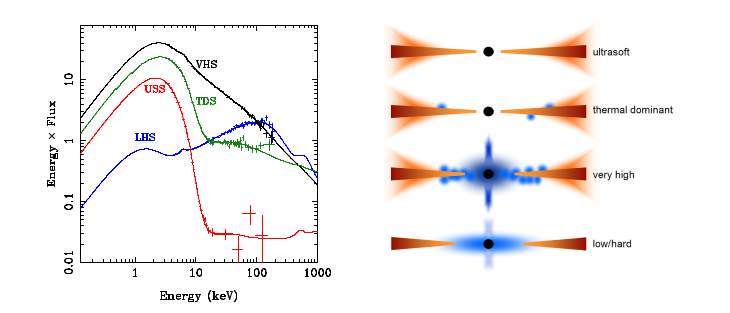
\includegraphics[width=0.8\linewidth]{SpectralTypes}
		\caption{Il grafico a sinistra mostra una serie di stati raccolti dall'esplosione (outburst) del 2005 di GRO J1655-40, mentre la figura a destra mostra in maniera semplificata una serie di possibili variazioni sul modello di accrescimento, con diversi contributi dal disco, modelli della sua regione interna, modelli del getto che potrebbe aver emesso, comportamento delle regioni sopra il disco e di un possibile vento.}
		\label{fig:SpectralTypes}
	\end{figure}
	
	Quindi, sono ora disponibili due modelli di flusso di accrescimento stabile, il disco sottile e il flusso disordinato e otticamente sottile, con almeno tre diversi tipi spettrali da spiegare. Flussi caldi insieme al modello di disco troncato sembrano essere sufficienti a descrivere le proprietà della componente dura dello spettro, mentre il modello a disco sembra descrivere meglio le proprietà ad alte $L/L_{edd}$. Ad alte luminosità il disco dovrebbe estendersi verso l'ISCO, ma anche nel caso di spettri morbidi è sempre	visibile una coda ad alte energie. Deve esserci quindi una sorta di dissipazione otticamente sottile che conviva con un flusso maggiormente disposto come un disco. Questo potrebbe essere legato all'evenienza che parte del disco si trovi in uno stato analogo a quello del flusso caldo disordinato, ma con proprietà modificate dall'intenso raffreddamento Compton (Esin 1997, Janiuk, Zycki e Czerny 2000) e conduzione termica (Rozanska e Czerny 2000, Liu, Meyer e Meyer-Hofmeister 2005). Esistono alternative a questi flussi regolari in modelli in cui la dissipazione di energia è intrinsecamente molto disomogenea, forse a causa della ricongiunzione magnetica di tubi di flusso emergenti dalla superficie del disco (Galeev, Rosner e Vaiana 1979, MRI: Hawley e Balbus 2002).

\newpage
\section{Conclusione}

	Anche se la ricerca si è concentrata sull'accrescimento nelle situazioni a gravità molto intensa, non ha senso considerare i risultati ottenuti dipendenti dalla scala di grandezza. Anzi, ha senso dire che ogni osservazione in situazioni estreme permetta di delineare un modello di accrescimento valido ovunque.
	
	Un altro risvolto interessante dello studio dell'accrescimento sbocciato negli ultimi anni è che lo studio dei sistemi in regime ultra-critico rispetto al limite di Eddington, potrebbe avere valenza cosmologia e spiegare come i venti stellari abbiano contribuito alla formazione delle prime pulsar nell'universo antico.
	
\newpage
\renewcommand{\bibpreamble}{Per regioni di coerenza interna al testo e di visione ordinata degli argomenti, ho cercato di affrontarli seguendo il più delle volte la traccia e le argomentazioni come sono presentatate sul testo di \textit{Frank, King e Raine}\cite{FrankKingRaineAccretionPower}, manuale di riferimento per quanto riguarda le teorie dell'accrescimento.
	
	Sono stati fondamentali anche alcune  \textit{review} di \textit{King}\cite{King2012} e \textit{Pringle}\cite{Pringle1981}, che sintetizzano efficacemente l'argomento dell'accrescimento e permettono di avere una visione di insieme dei risultati ottenuti.
	
	E' stato fondamentale per la mia comprensione dello sviluppo delle teorie, l'analisi e la lettura degli articoli originali sui modelli di disco di accrescimento intorno ai corpi compatti.
	Ho lavorato quindi anche con gli articoli seminali di \textit{Pringle}, \textit{Reese}, \textit{Shakura}, \textit{Sunyaev} e \textit{Pacholczyk}\cite{PringleReese1972}\cite{PringleReesPacholczyk1973}\cite{ShakuraSunyaev1973} e la splendida analisi del lavoro nella fondazione della teoria di accrescimento di Zeldovich svolta da Shakura quest'anno\cite{ShakuraZeldovich2018}.
	
	Per quanto riguarda in particolare l'argomento della tesi, ovvero l'instabilità nelle regioni dominate dalla pressione radiativa nel modello del disco di accrescimento, ho fatto riferimento al primissimo lavoro a riguardo di \textit{Lightman} ed \textit{Eardley}\cite{LightmanEardley1974} e ad articoli successivi che estendono, propongono alternative, ne analizzanoi risultati o li computano. Questi sono stati scritti da \textit{Shakura} e \textit{Sunyaev}\cite{ShakuraSunyaev1976}, \textit{Shapiro} con gli stessi \textit{Lightman} ed \textit{Eardley}\cite{ShapiroLightmanEardley1976}, \textit{Taam} e \textit{Lin}\cite{TaamLin1984} e \textit{Teresi}, \textit{Molteni} e \textit{Toscano}\cite{TeresiMolteniToscano2004}.
	
	Per quanto riguarda i risultati osservativi nei sistemi binari ho fatto riferimento all'immeno articolo di review del 2007 sulle osservazioni dei primi anni '00 firmato da Done, Gierlinski e Kubota \cite{DoneGierlinskiKubota2007}
	
	Per tutti gli aspetti non strettamente legati all'accrescimento ho fatto riferimento a tre manuali: il \textit{Maoz}\cite{MaozNutshell} e il \textit{Prialnik} \cite{PrialnikStellarStructureEvolution} per i cenni sulla struttura dei corpi compatti e il \textit{Ghisellini}\cite{GhiselliniRadiativi} per quanto riguarda i processi radiativi.}
	
\begin{thebibliography}{9}

	\bibitem{DoneGierlinskiKubota2007} 
	C. Done, M. Gierlinski, A. Kubota
	"Modelling the behaviour of accretion flows in X-ray binaries. Everything you wanted yo know about accretion but were afraid to ask"\\
	\textit{arXiv}:0708.0148v1

	\bibitem{FrankKingRaineAccretionPower} 
	J. Frank, A. King, D. Raine
	"Accretion Power in Astrophysics"\\
	\textit{Cambridge University Press}, 2002 (III ed.)
	
	\bibitem{King2012} 
	A. King 
	"Accretion Disc Theory since Shakura and Sunyaev"\\
	\textit{arXiv}: 1201.2060v1\\
	\textit{to appear in proceedings of 'The Golden Age of Cataclysmic Variables', Memorie Società Astronomica Italiana, 2012 (F. Giovannelli and L. Sabau-Graziati eds.)}
	
	\bibitem{GhiselliniRadiativi} 
	G. Ghisellini
	"Radiative Processes in High Energy Astrophysics"\\
	\textit{Springer}, 2013
	
	\bibitem{LightmanEardley1974} 
	A. P. Lightman, D. M. Eardley 
	"Black Holes in Binary Systems: Instability of Fisk Accretion"\\
	\textit{Astrop. Journal} 187, L1-L3, 1974 January 1
	
	\bibitem{MaozNutshell} 
	D. Maoz
	"Astrophysics in a nutshell"\\
	\textit{Princeton University Press}, 2007
	
	\bibitem{PrialnikStellarStructureEvolution} 
	D. Prialnik
	"An Introduction to the Theory of Stellar Structure and Evolution"\\
	\textit{Cambridge University Press}, 2000
	
	\bibitem{Pringle1981} 
	J. E. Pringle 
	"Accretion Discs in Astrophysics"\\
	\textit{Ann. Rev. Astron. Astrphys.} 1981, 19:137-62
	
	\bibitem{PringleReese1972} 
	J. E. Pringle, M. J. Rees
	"Accretion Discs Model for Compact X-Ray Sources"\\
	\textit{Astron. \& Astrphys.} 21, 1-9 (1972)
	
	\bibitem{PringleReesPacholczyk1973} 
	J. E. Pringle, M. J. Rees, A. G. Pacholczyk
	"Accretion onto Massive Black Holes"\\
	\textit{Astron. \& Astrphys.} 29, 179-184 (1973)
	
	\bibitem{ShakuraSunyaev1973}
	N. I. Shakura, R. A. Sumyaev 
	"Black Holes in Binary Systems. Observational Appearance"\\
	\textit{Astron. \& Astrophys.} 24, 337-355 (1973)
	
	\bibitem{ShakuraSunyaev1976}
	N. I. Shakura, R. A. Sumyaev 
	"A Theory of the Instability of Disk Accretion on to Black Holes and the Variability of Binary X-Ray Sources, Galactic Nuclei and Quasars"\\
	\textit{Mon. Not. R. astr. Soc.} (1976) 175, 613-632
	
	\bibitem{ShakuraZeldovich2018}
	N. I. Shakura
	"Ya. B. Zeldovich and foundation of the accretion theory"\\
	\textit{arXiv}: 1809.1137v1
	
	\bibitem{ShapiroLightmanEardley1976} 
	S. L. Shapiro, A. P. Lightman, D. M. Eardley 
	"A Two-Temperature Disk Model for Cygnus X-1 Structure and Spectrum"\\
	\textit{Astrop. Journal} 187-199, 1976 February 15
	
	\bibitem{TaamLin1984} 
	R. E. Taam, D. N. C. Lin 
	"The Evolution of the Inner Regions of Viscous Accretion Disks Surrounding Neutron Stars"\\
	\textit{Astrop. Journal} 287, 761-768 1984 December 15
	
	\bibitem{TeresiMolteniToscano2004} 
	V. Teresi, D. Molteni, E. Toscano 
	"SPH Simulations of Shakura-Sunyaev Instability at Intermediate Accretion Rates"\\
	\textit{Mon. Not. R. Astron. Soc.} 348, 361-367 (2004)
\end{thebibliography}

\end{document}
